\documentclass[a4paper,12pt,bibliography=totoc]{scrartcl}
\usepackage[utf8]{inputenc}
\usepackage[ngerman]{babel}
\usepackage{amsmath,amssymb,amsthm}
\usepackage{graphicx}
\usepackage{float}
\usepackage{microtype}
\usepackage[onehalfspacing]{setspace}
\setlength{\parindent}{0pt}
%Zitieren
%========
%deutsche Anführungszeichen mit
\usepackage[babel,german=quotes]{csquotes}
\usepackage[style=alphabetic,natbib=true,backend=biber]{biblatex}
\bibliography{literatur.bib}

%Verlinkungen
%============
\usepackage[colorlinks,
pdfpagelabels,
pdfstartview = FitH,
bookmarksopen = true,
bookmarksnumbered = true,
linkcolor = black,
plainpages = false,
hypertexnames = false,
citecolor = black] {hyperref}

%Seitenränder
%============
\usepackage{geometry}
\geometry{a4paper, top=20mm, left=40mm, right=20mm, bottom=30mm,
	headsep=10mm, footskip=10mm}

%Nummerierung der Sätze, Lemmas, Definitionen und Bemerkungen
%============================================================
\newtheorem{theorem}{Satz}[section]
\newtheorem{lemma}[theorem]{Lemma}
\newtheorem{bem}[theorem]{Bemerkung}
\newtheorem{defi}[theorem]{Definition}
\newtheorem{bsp}[theorem]{Beispiel}
\newcommand{\OR}[1]{{\mathcal{O}(\mathbb{R}^#1)}}
\DeclareMathOperator{\Span}{span}

\begin{document}

\begin{titlepage}
\begin{center}

% Upper part of the page. The '~' is needed because \\
% only works if a paragraph has started.
% \includegraphics[width=0.15\textwidth]{./logo}~\\[1cm]

\textsc{\LARGE Universität Duisburg-Essen}\\
\textsc{Fakultät für Mathematik}\\[6.8cm]

\textsc{\Large Bachelorarbeit}\\[0.5cm]

% Title
{ \huge \bfseries Endliche Untergruppen der orthogonalen Gruppen im zwei- und dreidimensionalem Raum \\[0.8cm] }

% Author and supervisor
\begin{minipage}{0.4\textwidth}
\begin{flushleft} \large
\emph{Autor:}\\
Mike Barkmin
\end{flushleft}
\end{minipage}
\begin{minipage}{0.4\textwidth}
\begin{flushright} \large
\emph{Betreuer:} \\
Dr. Ingo Janiszczak
\end{flushright}
\end{minipage}

\vfill

% Bottom of the page
{\large \today}
%\setcounter{tocdepth}{1}
%\tableofcontents
\end{center}
\end{titlepage}

\setcounter{tocdepth}{2}
\tableofcontents
\newpage
\section{Einleitung}
%Eine Einleitung, in der Sie das Thema der Arbeit, die Einordnung in den wissenschaftlichen Kontext, die Geschichte der Fragestellung und die genaue Art Ihrer Bearbeitung (etwa: Ausarbeitung mit eigenem Beispiel, Computersimulation zu Beispiel xy, Ausarbeitung und Beweis des Satzes yz etc) besprechen. Diese Einleitung richtet sich an einen mathematisch vorgebildeten, aber mit der genauen Thematik nicht notwendigerweise vertrauten Leser. Sie geben auch in der Einleitung noch einmal die Textvorlagen an, die Sie verwendet haben.
Die Betrachtung der orthogonalen Gruppe stellt aus didaktischer Sicht eine Brücke zwischen der Linearen Algebra und der Algebra dar: Sie ermöglicht die Anwendung und Interpretation von Begriffen aus der Linearen Algebra und fördert das Verständnis vom Gruppenbegriff durch den Umgang mit nicht-trivialen Gruppen und leistet damit Vorarbeit auf dem Gebiet der Algebra. Insbesondere bieten die orthogonalen Gruppen und ihre Aktionen auf geometrischen Objekten einen mathematischen Zugang zur Symmetrie, was sich wiederum positiv auf die Anschaulichkeit auswirkt.\\
Der Betrachtung der orthogonalen Gruppen im zwei- bzw. dreidimensionalen euklidischen Vektorraum wohnt damit sogar Potential für die Thematisierung im Fachunterricht Mathematik in der Sek. II inne.
%Die vorliegende Arbeit könnte in diesem Kontext beispielsweise als Basisliteratur für die Lehrkraft dienen. Einerseits sind die fachlichen Grundlagen mit Sätzen und Beweisen abgesichert, andererseits wurde Wert auf die Anschaulichkeit der Darstellung gelegt.\\
Zunächst werden wir die orthogonalen Abbildungen im zweidimensionalen Raum betrachten. Wir werden erstens sehen, dass dort jede orthogonale Abbildung eine Drehung oder eine Spiegelung ist. Zweitens können wir eine Klassifikation der endlichen Untergruppen der orthogonalen Gruppen vornehmen. Insbesondere stellen wir fest, dass wir Gruppen mit regulären Polygonen assoziieren können.\\
Darauf aufbauend betrachten wir im nächsten Kapitel die orthogonalen Abbildungen im dreidimensionalen Raum, wo wir neben Spiegelungen und Drehungen zusätzlich Drehspiegelungen unterscheiden können. An die Stelle der Polygone treten nun die regulären Polyeder im Abschnitt zu den Platonischen Körpern. Nach einem kurzen Exkurs zur Rezeption der Platonischen Körper in den Naturwissenschaften seit der Antike werden wir uns auf zwei Arten davon überzeugen, dass es nur fünf regelmäßige Polyeder geben kann. Wir bedienen uns dabei einmal elementargeometrischer Überlegungen, während wir beim zweiten Beweis auf Begriffe der Graphentheorie und den Eulerschen Polyedersatz zurückgreifen.\\
Wie auch im zweidimensionalen Raum nehmen wir eine Klassifikation der endlichen Untergruppen vor: Wir beginnen mit der Klassifikation der endlichen Drehgruppen und beschäftigen uns mit den Drehgruppen der platonischen Körpern. Eine selbstgeschriebene Web-Applikation visualisiert alle Drehungen der platonischen Körper. Schließlich erhalten wir die vollständige Liste der fünf endlichen Untergruppen von Drehungen.\\
Verallgemeinert wird das Resultat durch die Ausweitung der Klassifikation auf die endlichen orthogonalen Gruppen im letzten Unterkapitel. Im letzten Satz werden wir feststellen, dass wir zu jeder Untergruppe der orthogonalen Gruppe im dreidimensionalen Raum eine Klasse angeben können, zu der sie isomorph ist und diese Liste umfassend ist.
Als Literatur für diese Arbeit dient das Buch \enquote{Finite Reflection Groups} von L.C. Grove und C.T Benson.

\section{Orthogonale Abbildungen im zweidimensionalen Raum}
Sei $T$ aus $\OR{2}$, der Menge der orthogonalen Abbildungen, dann ist $T$ eindeutig durch die Bilder der Basisvektoren $e_1 = (1,0)$ und $e_2 = (0,1)$ bestimmt. Da $T$ aus $\OR{2}$ ist und somit längen- und orthogonalitätserhaltend ist, können wir einen Winkel $\theta$ zwischen $0$ und $2 \pi$ wählen, sodass gilt: Wenn $Te_1 = (\cos(\theta),\sin(\theta))$, dann ist $Te_2 = \pm (-\sin(\theta),\cos(\theta))$.
Wir müssen nun die zwei Fälle für $Te_2$ unterscheiden. Zunächst wollen wir uns mit dem positiven Fall beschäftigen. 

Wenn $Te_2 = + (-\sin(\theta),\cos(\theta))$, dann können wir eine geordnete orthogonale Basis $W$ wählen, sodass für die Abbildungsmatrix von $T$ zur Basis $W$ gilt:
$$A =\;_W\!(T)_W = \begin{pmatrix}
	\cos(\theta) && -\sin(\theta) \\
	\sin(\theta) && \cos(\theta)
\end{pmatrix} $$
Wir können erkennen, dass es sich um eine Rotation in der Ebene um den Ursprung mit Rotationswinkel $\theta$ handelt. Außerdem können wir erkennen, dass wegen dem Satz des Pythagoras gilt: $\det T = \cos^2(\theta) + \sin^2(\theta) = 1$.
Jetzt möchten wir uns mit dem negativen Fall beschäftigen und gehen ähnlich wie im positiven Fall vor.

Wenn $Te_2 = - (-\sin(\theta),\cos(\theta))$, dann können wir eine geordnete orthogonale Basis $U$ wählen, sodass für die Abbildungsmatrix von $T$ zur Basis $U$ gilt:
$$B =\;_U\!(T)_U = \begin{pmatrix}
	\cos(\theta) && \sin(\theta) \\
	\sin(\theta) && -\cos(\theta)
\end{pmatrix}.$$
In diesem Fall können wir erkennen, dass gilt: $\det T = -\cos^2(\theta) -\sin^2(\theta) = -(\cos^2(\theta) +\sin^2(\theta)) = -1$. Außerdem kann eine weitere Eigenschaft der Abbildungsmatrix festgestellt werden. Es gilt:
$$B^2 = \begin{pmatrix}
	\cos^2(\theta) + \sin^2(\theta) && 0 \\
	0 && \cos^2(\theta) + \sin^2(\theta)
\end{pmatrix} = \begin{pmatrix}
	1 && 0 \\
	0 && 1 
\end{pmatrix} = 1.
$$Wenn wir uns die Vektoren $x_1 = (\cos(\theta/2),\sin(\theta/2))$ und $x_2 = (-\sin(\theta/2),\cos(\theta/2))$ anschauen, dann können wir leicht sehen, dass diese Eigenvektoren von $B$ mit den Eigenwerten $1$ und $-1$ sind. Um das zu überprüfen, verknüpfen wir $B$ mit $x_1$ und erhalten mit Hilfe der Additionstheoreme folgende Gleichungskette:
\begin{align*}
	Bx_1 &= \begin{pmatrix}
		\cos(\theta) && \sin(\theta) \\
		\sin(\theta) && -\cos(\theta)
	\end{pmatrix} \begin{pmatrix}
		\cos(\theta/2) \\
		\sin(\theta/2)
	\end{pmatrix} = \begin{pmatrix}
		\cos(\theta)\cos(\theta/2)+\sin(\theta)\sin(\theta/2) \\
		\sin(\theta)\cos(\theta/2)-\cos(\theta)\sin(\theta/2)
	\end{pmatrix} \\ &= \begin{pmatrix}
		\cos(\theta - \theta/2) \\
		\sin(\theta - \theta/2)
	\end{pmatrix} = \begin{pmatrix}
		\cos(\theta/2) \\
		\sin(\theta/2)
	\end{pmatrix}.
\end{align*}
Demnach ist $x_1$ ein Eigenvektor zum Eigenwert $1$ von $B$. Genauso können wir überprüfen, ob $x_2$ ein Eigenvektor zum Eigenwert $-1$ von $B$ ist.
\begin{align*}
	Bx_2 &= \begin{pmatrix}
		\cos(\theta) && \sin(\theta) \\
		\sin(\theta) && -\cos(\theta)
	\end{pmatrix} \begin{pmatrix}
		-\sin(\theta/2) \\
		\cos(\theta/2)
	\end{pmatrix} = \begin{pmatrix}
		-\cos(\theta)\sin(\theta/2)+\sin(\theta)\cos(\theta/2) \\
		-\sin(\theta)\sin(\theta/2)-\cos(\theta)\cos(\theta/2)
	\end{pmatrix} \\ &= \begin{pmatrix}
		\sin(\theta - \theta/2) \\
		-\cos(\theta - \theta/2)
	\end{pmatrix} = \begin{pmatrix}
		\sin(\theta/2) \\
		-\cos(\theta/2)
	\end{pmatrix}.
\end{align*}
Wenn wir nun die Abbildungsmatrix $C$ von $T$ bezüglich der Basis $\{x_1,x_2\}$ bestimmen, dann erhalten wir
$$C = \begin{pmatrix}
	1 && 0 \\
	0 && -1
\end{pmatrix}.$$
Daraus können wir entnehmen, dass die orthogonale Abbildung $T$, wenn wir einen Vektor $x$ als Linearkombination von $x_1$ und $x_2$ wählen, $x$ auf sein Spiegelbild bezüglich der Geraden, die durch den Vektor $x_1$ aufgespannt wird, abgebildet wird. Solche orthogonalen Abbildungen nennen wir Spiegelungen an der Gerade $\langle x_1 \rangle$. Weiterhin können wir festhalten, dass für alle Vektoren $x$ aus der Ebene $\mathbb{R}^2$ gilt
$$Tx = x - 2(x,x_2)x_2.$$
Somit haben wir gezeigt, dass jede orthogonale Abbildung von $\mathbb{R}^2$ entweder eine Rotation oder eine Spiegelung ist.

\subsection{Klassifikation der endlichen orthogonalen Gruppen}
Nachdem wir uns mit den orthogonalen Abbildungen im zweidimensionalen Raum vertraut gemacht und ihre besonderen Eigenschaften kennen gelernt haben, möchten wir uns mit der Klassifizierung von endlichen Untergruppen der orthogonalen Gruppe befassen. 

Der nachfolgende Satz \ref{klassO(R2)} teilt die endlichen Untergruppen der orthogonalen Gruppe in zwei Klassen ein. Einmal in die Untergruppen vom Typ der zyklischen Gruppe und in die vom Typ der Diedergruppe.
\begin{theorem}\label{klassO(R2)}
	Sei $\mathcal{G}$ eine endliche Untergruppe von $\OR{2}$, dann ist $\mathcal{G}$ entweder eine zyklische Gruppe $\mathcal{C}^n_2$ oder eine Diedergruppe $\mathcal{H}^n_2$ für $n \in \mathbb{N}$
\end{theorem}
Bevor wir diesen Satz beweisen sollten wir uns vorher die Definitionen der Diedergruppe, der zyklischen Gruppe und der Nebenklassen anschauen und nachvollziehen.
\begin{defi}[Zyklische Gruppe]
	Eine Gruppe $\mathcal{C}$ heißt zyklisch, wenn sie ein Element $A$ enthält, sodass für jedes Element $B$ von $\mathcal{C}$ ein $n \in \mathbb{Z}$ existiert, sodass $A^n = B$. Außerdem gilt, dass $\mathcal{C}$ die einzige Untergruppe von $\mathcal{C}$ ist, die $A$ enthält. Dann nennen wir $A$ den Erzeuger von $\mathcal{C}$ und können schreiben $\mathcal{C} = <A>$.
\end{defi}
Damit wir die Definition der zyklischen Gruppe besser verstehen können, werden wir uns eine Gruppe anschauen und überprüfen, ob diese zyklisch ist. 

Wir nehmen uns die Gruppe $\mathcal{C}_4$. Diese Gruppe enthält alle möglichen Drehungen der Ebene die ein Quadrat in sich überführen. Also besteht die Gruppe wie in der Abbildung \ref{fig:zyklische_gruppe_c4} zu erkennen ist aus den Drehungen um $90^{\circ}$, $180^{\circ}$, $270^{\circ}$ und $0^{\circ}$, da Drehwinkel immer Modulo $360^{\circ}$ gerechnet werden.
\begin{figure}[H]
	\centering
	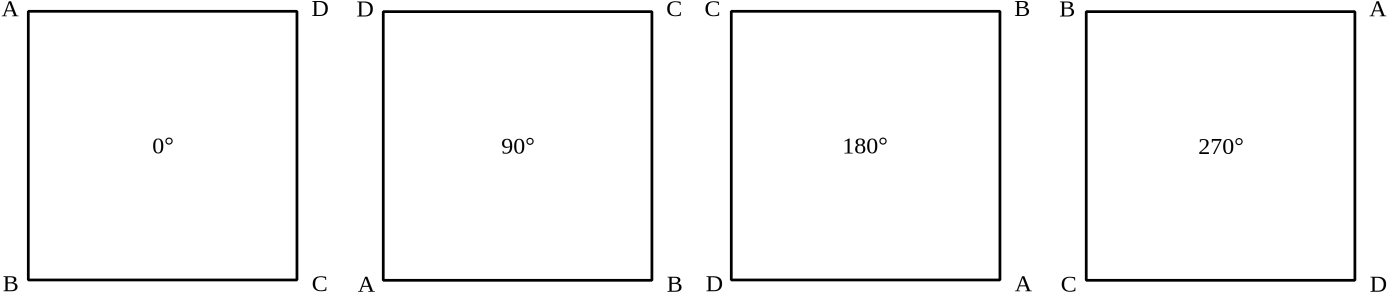
\includegraphics[width=1\linewidth]{grafiken/zyklische_gruppe_c4}
	\caption{Grafische Darstellung der Elemente von $\mathcal{C}_4$}
	\label{fig:zyklische_gruppe_c4}
\end{figure}
Um zu überprüfen ob diese Gruppe zyklisch ist, können wir nun versuchen die Definition der zyklischen Gruppe anzuwenden. Wählen wir uns zum Beispiel das Element A, die Drehung um $90^{\circ}$. Wir müssen nun zeigen, dass wir jedes andere Element der Gruppe mit dem Element A darstellen können. Dies können wir natürlich. Damit wir die Drehung um $180^{\circ}$ darstellen können müssen wir A mit sich selber verknüpfen. Um $270^{\circ}$ darstellen müssen wir A dreimal mit sich selber verknüpfen. Da wir nun alle Element der Gruppe $\mathcal{C}_4$ mit A darstellen können, haben wir herausgefunden, dass die Gruppe eine zyklische Gruppe mit Erzeuger A, der Drehung um $90^{\circ}$ ist. \par\smallskip
Wenn wir auch Spiegelungen zulassen, dann erhalten wir im Falle von regelmäßigen Polygonen eine Diedergruppe.
\begin{defi}[Diedergruppe]
	Eine Gruppe $\mathcal{H}$ ist eine Diedergruppe, wenn sie die Isometriegruppe eines regelmäßigen $n$-Ecks in der Ebene ist. Sie besteht dann aus $n$ Drehungen und $n$ Spiegelungen, also aus insgesamt $2n$ Elementen.
\end{defi}
Auch für Diedergruppen möchten wir uns ein Beispiel, dazu können wir uns dem vorherigen Beispiel bedienen und wie schon erwähnt noch Spiegelungen der Gruppe hinzufügen, die das Viereck in sich selber überführen, hinzunehmen.
\begin{figure}[H]
	\centering
	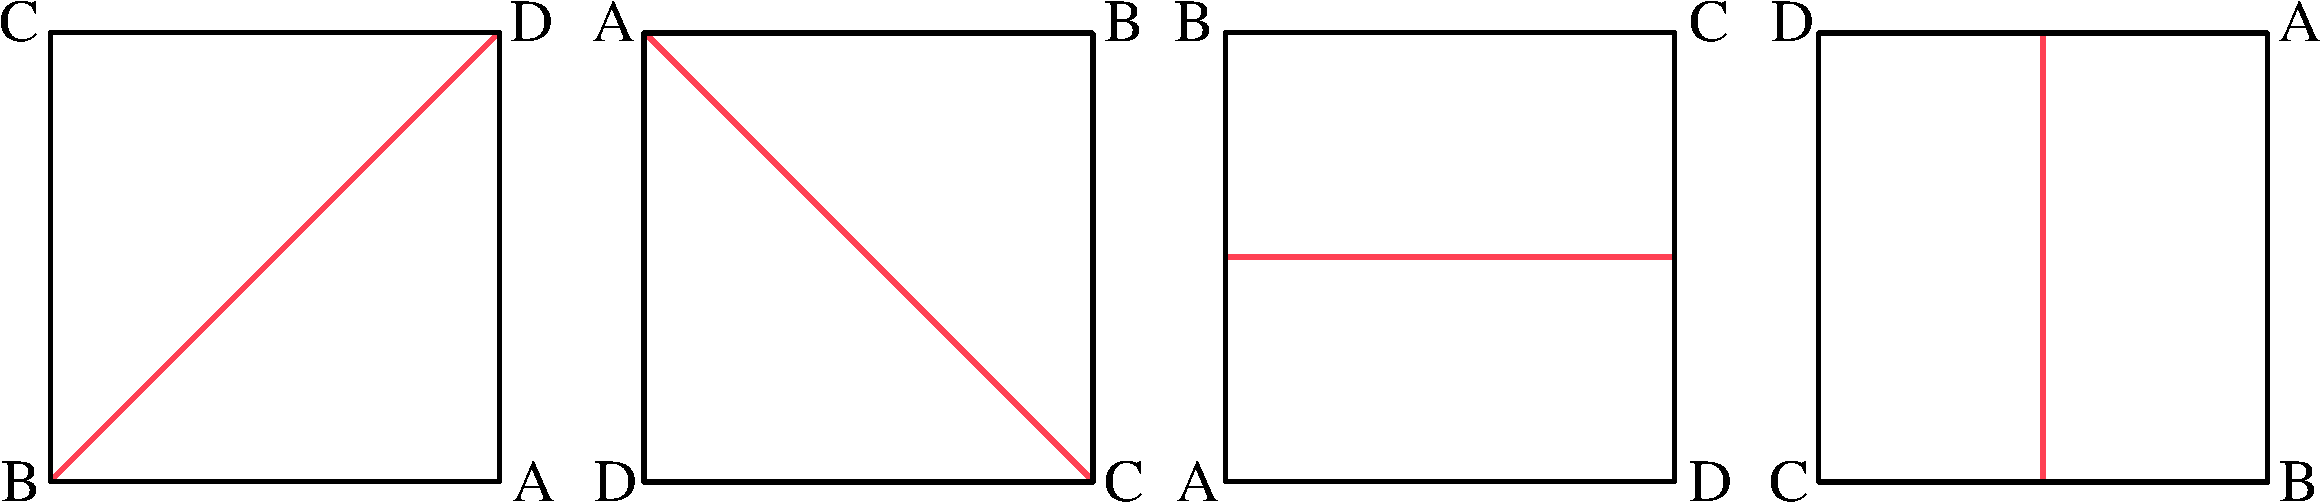
\includegraphics[width=1\linewidth]{grafiken/dieder_gruppe}
	\caption{Grafische Darstellung der Elemente von $\mathcal{D}_4$}
	\label{fig:zyklische_gruppe_d4}
\end{figure}
Wie in der Abbildung \ref{fig:zyklische_gruppe_d4} zu sehen ist, kommen vier weitere Elemente zu der Gruppe hinzu. Diese vier Spiegelungen zusammen mit den vier Rotationen vom vorherigen Beispiel bilden die Diedergruppe $\mathcal{D}_4$. Diese Gruppe besitzt zwei Erzeuger, zum einen den Erzeuger der zyklischen Gruppe $\mathcal{C}_4$ und zum anderen eine der vier Spiegelungen. 
\begin{defi}[Linksnebenklasse]
	Zu einer Untergruppe $\mathcal{H} \subseteq \mathcal{G}$ heißt eine Teilmenge der Form $g\mathcal{H} = \{gh|h\in\mathcal{H}\}$ mit $g \in G$ eine Linksnebenklasse. Die Anzahl der Linksnebenklassen heißt der Index von $\mathcal{H}$ in $\mathcal{G}$.
\end{defi}
Als Beispiel nehmen wir uns die Diedergruppe $\mathcal{D}_4$, mit der wir uns schon besser vertraut gemacht haben. Die zyklische Gruppe $\mathcal{C}_4$ ist eine Untergruppe der Diedergruppe mit Index 2. Es ist leicht zu sehnen, dass die zyklische Gruppe eine Untergruppe der Diedergruppe ist, wir können die zyklische Gruppe auch als Linksnebenklasse auffassen, indem wir die Gruppe von Links mit Einheitsmatrix verknüpfen. Eine zweite Linksnebenklasse die wir finden können, entsteht durch die Verknüpfung einer beliebigen Spiegelung der Diedergruppe mit der zyklischen Gruppen. Wenn wir nun beide Linksnebenklassen miteinander verbinden erhalten wir die vollständige Diedergruppe. Daher hat die zyklische Gruppe in der Diedergruppe den Index 2. \par\smallskip
Da wir nun wichtige Definitionen für Satz \ref{klassO(R2)} uns angeschaut und anhand von Beispiel versucht haben zu verstehen, können wir nun mit dem Beweis des Satzes beginnen. 
\begin{proof}
	 Zunächst wollen wir zeigen, dass wenn wir eine beliebige endliche Untergruppe von $\OR{2}$ wählen, die nur Rotationen enthält, dass diese vom Typ einer zyklischen Gruppen seien muss. \par\smallskip  
	 Sei $\mathcal{G}$ eine beliebige endliche Untergruppe von $\OR{2}$. Wir nehmen an, dass $\mathcal{H} \leq \mathcal{G}$ eine Untergruppe in $\mathcal{G}$ ist, die die Menge aller Rotationen in $\mathcal{G}$ enthält. 
	 
	 Wir wollen zeigen, dass $\mathcal{H}$ zyklisch sein muss. Für $|\mathcal{H}|=1$ ist dieses bereits klar. Wenn $|\mathcal{H}| \neq 1$ wählen wir eine Drehung $R \in \mathcal{H}$, sodass $R \neq E_2$ und der Drehwinkel $\theta(R)$ minimal ist. Wenn wir jetzt eine weitere Drehung $T \in \mathcal{H}$ nehmen, dann können wir ein $m \in \mathbb{Z}$ finden, sodass \begin{align*}
	 &m \theta(R)\leq\theta(T)<(m+1)\theta(R) \\
	 \Leftrightarrow \ &0 \leq \theta(T)-m\theta(R)<\theta(R) \\
	 \Leftrightarrow \ &0 \leq \theta(TR^{-m})<\theta(R)                                                                                                                                                                                                                                                                                                                                                           
	 \end{align*}
	 Da wir $\theta(R)$ minimal gewählt haben, gilt $\theta(TR^{-m})=0$. Also muss $TR^{-m}=E_2$ sein und es folgt $T=R^{m}$. Demnach ist $\mathcal{H}$ zyklisch mit $\mathcal{H}=<R>$ ($R$ ist Erzeuger von $\mathcal{H}$). Damit folgt auch, dass $\theta(R)=\frac{2}{n}\pi$, wenn $n=|\mathcal{H}|$. Wenn $\mathcal{G} = \mathcal{H}$ gilt, dann haben wir gezeigt, dass $\mathcal{G}$ zyklisch ist und wir bezeichnen $\mathcal{G}$ mit $\mathcal{C}^n_2$.
	 
	 Als nächstes nehmen wir dann an, dass $\mathcal{G} \neq \mathcal{H}$ und wählen eine Spiegelung $S \in \mathcal{G}$. Nun wählen wir eine weitere beliebige Spiegelung $T \in \mathcal{G}$ mit $T \neq S$, dann gilt $\det(ST)=\det(S)\det(T)=1$. Deshalb gilt $ST \in \mathcal{H}$ und es handelt sich bei $ST$ um eine Drehung. Dann gilt $T \in S\mathcal{H}$, da $S^{-1}=S$. So gilt, dass $\mathcal{H}$ eine Untergruppe von $\mathcal{G}$ mit Index $2$ ist und $\mathcal{H}=<R>$. Dann gilt $\mathcal{G}=<R,S>$ $=\{E_2,R,\dots \ ,R^{n-1},S,SR,\dots ,SR^{n-1}$\} und $|\mathcal{G}|=2n$. Da $RS$ eine Spiegelung ist, gilt $(RS)^2=E_2$ und $RS=SR^{-1}=SR^{n-1}$, damit sind alle Verknüpfungen in $\mathcal{G}$ festgelegt. Die Gruppe $\mathcal{G}$ bezeichnen wir mit $\mathcal{H}^n_2=<S,R>$ (Die Diedergruppe von Ordnung 2n).
\end{proof}
\section{Orthogonale Abbildungen im dreidimensionalen Raum}
In den folgenden Abschnitten gehen wir von $V= \mathbb{R}^3$ aus.\\
Wir betrachten nacheinander Drehungen, Spiegelungen und Drehspiegelungen und charakterisieren diese, indem wir ihre Eigenschaften nennen und durch Beweis begründen. 
\begin{theorem}
Sei $T$ eine Drehung aus der orthogonalen Gruppe $\OR{3}$, dann hat $T$ eine fixierte Drehachse, die durch den Eigenvektor $x$ von $T$ zum Eigenwert 1 eindeutig festgelegt ist. 
Wenn wir $T$ auf die durch $x^{\perp}$ eindeutig festgelegte Ebene $\mathcal{P}$ einschränken, ist $T$ eine Drehung im zweidimensionalen Raum $\mathbb{R}^2$. 
\end{theorem}
\begin{proof}
Zunächst wollen wir klären, wie der Eigenwert 1 zustande kommt:
 Angenommen $T$ ist eine Drehung in $\OR{3}$ und $\lambda_1,\lambda_2,\lambda_3$ sind Eigenwerte von $T$, dann muss mindestens einer der Koeffizienten aus $\mathbb{R}$ sein, da nach dem Zwischenwertsatz aus der Analysis ein reelles Polynom dritten Grades mindestens eine reelle Nullstelle besitzt. Sei $\lambda_1$ (ggf. nach Umbenennung) aus $\mathbb{R}$, dann können $\lambda_2$ und $\lambda_3$ nur folgende Werte annehmen, da $\det(T)=\lambda_1\lambda_2\lambda_3=1$.
 \begin{align}
  \lambda_1=1, \lambda_2=\lambda_3=\pm1 \\
  \lambda_1=1, \lambda_2=\overline{\lambda_3}\notin \mathbb{R}
 \end{align}
Für uns ist nur der Eigenwert $1$ interessant, dieser ist aber in beiden Fällen vorhanden.\\
Es bleibt zu nachzuweisen, weshalb $\mathcal{T}|_\mathcal{P}$ eine Drehung in der Ebene $\mathcal{P}$ ist.
Sei $x$ ein Eigenvektor zum Eigenwert $1$, dann gilt nach der Definition eines Eigenvektors: $x=T^{-1}Tx=T^{-1}x$. Daraus können wir folgende Gleichungskette ableiten: $0=(x^{\perp},x)=(x^{\perp},T^{-1}x)=(Tx^{\perp},x)$ und direkt ablesen, dass $\mathcal{P}=x^{\perp}$ invariant ist unter $T$. Betrachten wir nun die Determinate der Einschränkung $T|_\mathcal{P}$, dann gilt $\det(T|_\mathcal{P})=1$, wegen $\det(T|_\mathcal{P}) = \lambda_2\lambda_3$ und $\lambda_2,\lambda_3$ wie oben.
\end{proof}
Die Eigenschaften der Spiegelungen in $\OR{3}$ fassen wir in einer Bemerkung zusammen:
\begin{bem}
Eine Spiegelung $S$ an der Ebene $\mathcal{P}$ ist eine Abbildung, für die gilt, dass $Sx=x$ für alle $x \in \mathcal{P}$. Die $y$ aus dem orthogonalen Komplement $P^{\perp}$ der Ebene $\mathcal{P}$ werden auf ihr Negatives abgebildet, kurz $Sy=-y$ für alle $y\in \mathcal{P}$.\\
Für alle Vektoren $z \in \mathbb{R}^3$ gibt es einen Einheitsvektor $r$ aus $P^{\perp}$, sodass die Abbildungsvorschrift $Sz = z -2(z,r)r$ gilt.\\
Nach Wahl einer geeigneten Basis $\{r, x_2, x_3\}$, wobei $\{x_2, x_3\}$ Basis der Spiegelebene $\mathcal{P}$ ist, kann die Spiegelung $S$ durch die Matrix $A$ dargestellt werden.
\begin{center}
  $A= \begin{pmatrix}
        -1 && 0 && 0 \\
        0 && 1 && 0 \\
        0 && 0 && 1 
       \end{pmatrix}$
 \end{center}
 \end{bem}
 Zweimaliges Spiegeln eines Vektors $z$ aus $\mathbb{R}^3$ überführt den Vektor wieder in sich selbst wegen: $A^2 = S^2 = E_3 = id$.\\
 Zuletzt betrachten wir Drehspiegelungen als Kombination von Spiegelung und Drehung.
 \begin{theorem}
 Sei $T\in\OR{3}$ mit $\det T = -1$. Dann ist $T$ eine Drehspiegelung mit Spiegelebene $\mathcal{P}$ und Drehachse $\mathcal{P}^{\perp}$.
 \end{theorem}
 Der Beweis verläuft ähnlich wie oben.
 \begin{proof}
 Diesmal sei $T$ eine Spiegelung aus $\OR{3}$ und $\lambda_1,\lambda_2, \lambda_3$ die Eigenwerte von $T$. Wie oben gibt es unter der Voraussetzung, dass $\lambda_1 \in \mathbb{R}$  und $\det T = \lambda_1\lambda_2\lambda_3=-1$ gilt, nur zwei mögliche Fälle:
 \begin{align}
   \lambda_1=-1, \lambda_2=\lambda_3=\pm1 \\
   \lambda_1=-1, \lambda_2=\overline{\lambda_3}\notin \mathbb{R}
  \end{align}
 Sei von nun an $x$ ein Eigenvektor zum Eigenwert $\lambda_1=-1$ und $\mathcal{P}$ das orthogonale Komplement $x^{\perp}$. Dass die Einschränkung $T|_\mathcal{P}$ eine Drehung in der Ebene $\mathcal{P}$ ist, wissen wir wegen $\det(T|_\mathcal{P}) = \lambda_2\lambda_3=1.$
 \end{proof}
 Wir wählen nun eine geeignete Basis $\{x_1,x_2\}$ zu $\mathcal{P}$, sodass wir $T$ darstellen können durch die Matrix $A$
 \begin{center}
   $A= \begin{pmatrix}
         -1 && 0 && 0 \\
         0 && \cos(\theta) && -\sin(\theta) \\
         0 && \sin(\theta) && \cos(\theta) 
        \end{pmatrix}$.
  \end{center}
 Die Darstellung als Produkt von einer Drehung und einer Spiegelung verdeutlicht den dargelegten Zusammenhang:
 \begin{center}
  $A=\begin{pmatrix}
            1 && 0 && 0 \\
            0 && \cos(\theta) && -\sin(\theta) \\
            0 && \sin(\theta) && \cos(\theta)
           \end{pmatrix} 
           \begin{pmatrix}
            -1 && 0 && 0 \\
            0 && 1 && 0 \\
            0 && 0 && 1
           \end{pmatrix}$.  
 \end{center}




\subsection{Platonische Körper}
In den vorherigen Kapiteln haben wir uns mit der Klassifizierung der endlichen Untergruppen der orthogonalen Gruppen im Zweidimensionalen beschäftigt. Dabei haben wir feststellen können, dass es für die Klassifizierung ausreicht nur Gruppen zu betrachten, die zu regulären Polygonen gehören, wie zum Beispiel die Gruppe $\mathcal{C}_4$, die zu einem Quadrat gehört. Da wir uns nun damit beschäftigen wollen, wie wir die endlichen Untergruppen der orthogonalen Gruppe im Dreidimensionalen klassifizieren können, liegt es nahe sich mit regulären Polyedern zu befassen.\\
Wir beginnen mit einigen Definitionen:
\begin{defi}[Einfaches Polyeder]
	Ein Polyeder heißt einfach, wenn seine Oberfläche sich stetig in eine Kugelfläche überführen lässt, das heißt einfache Polyeder haben keine \enquote{Löcher}. \citep[211]{Mainzer1988}
\end{defi}
\begin{figure}[H]
    \centering
    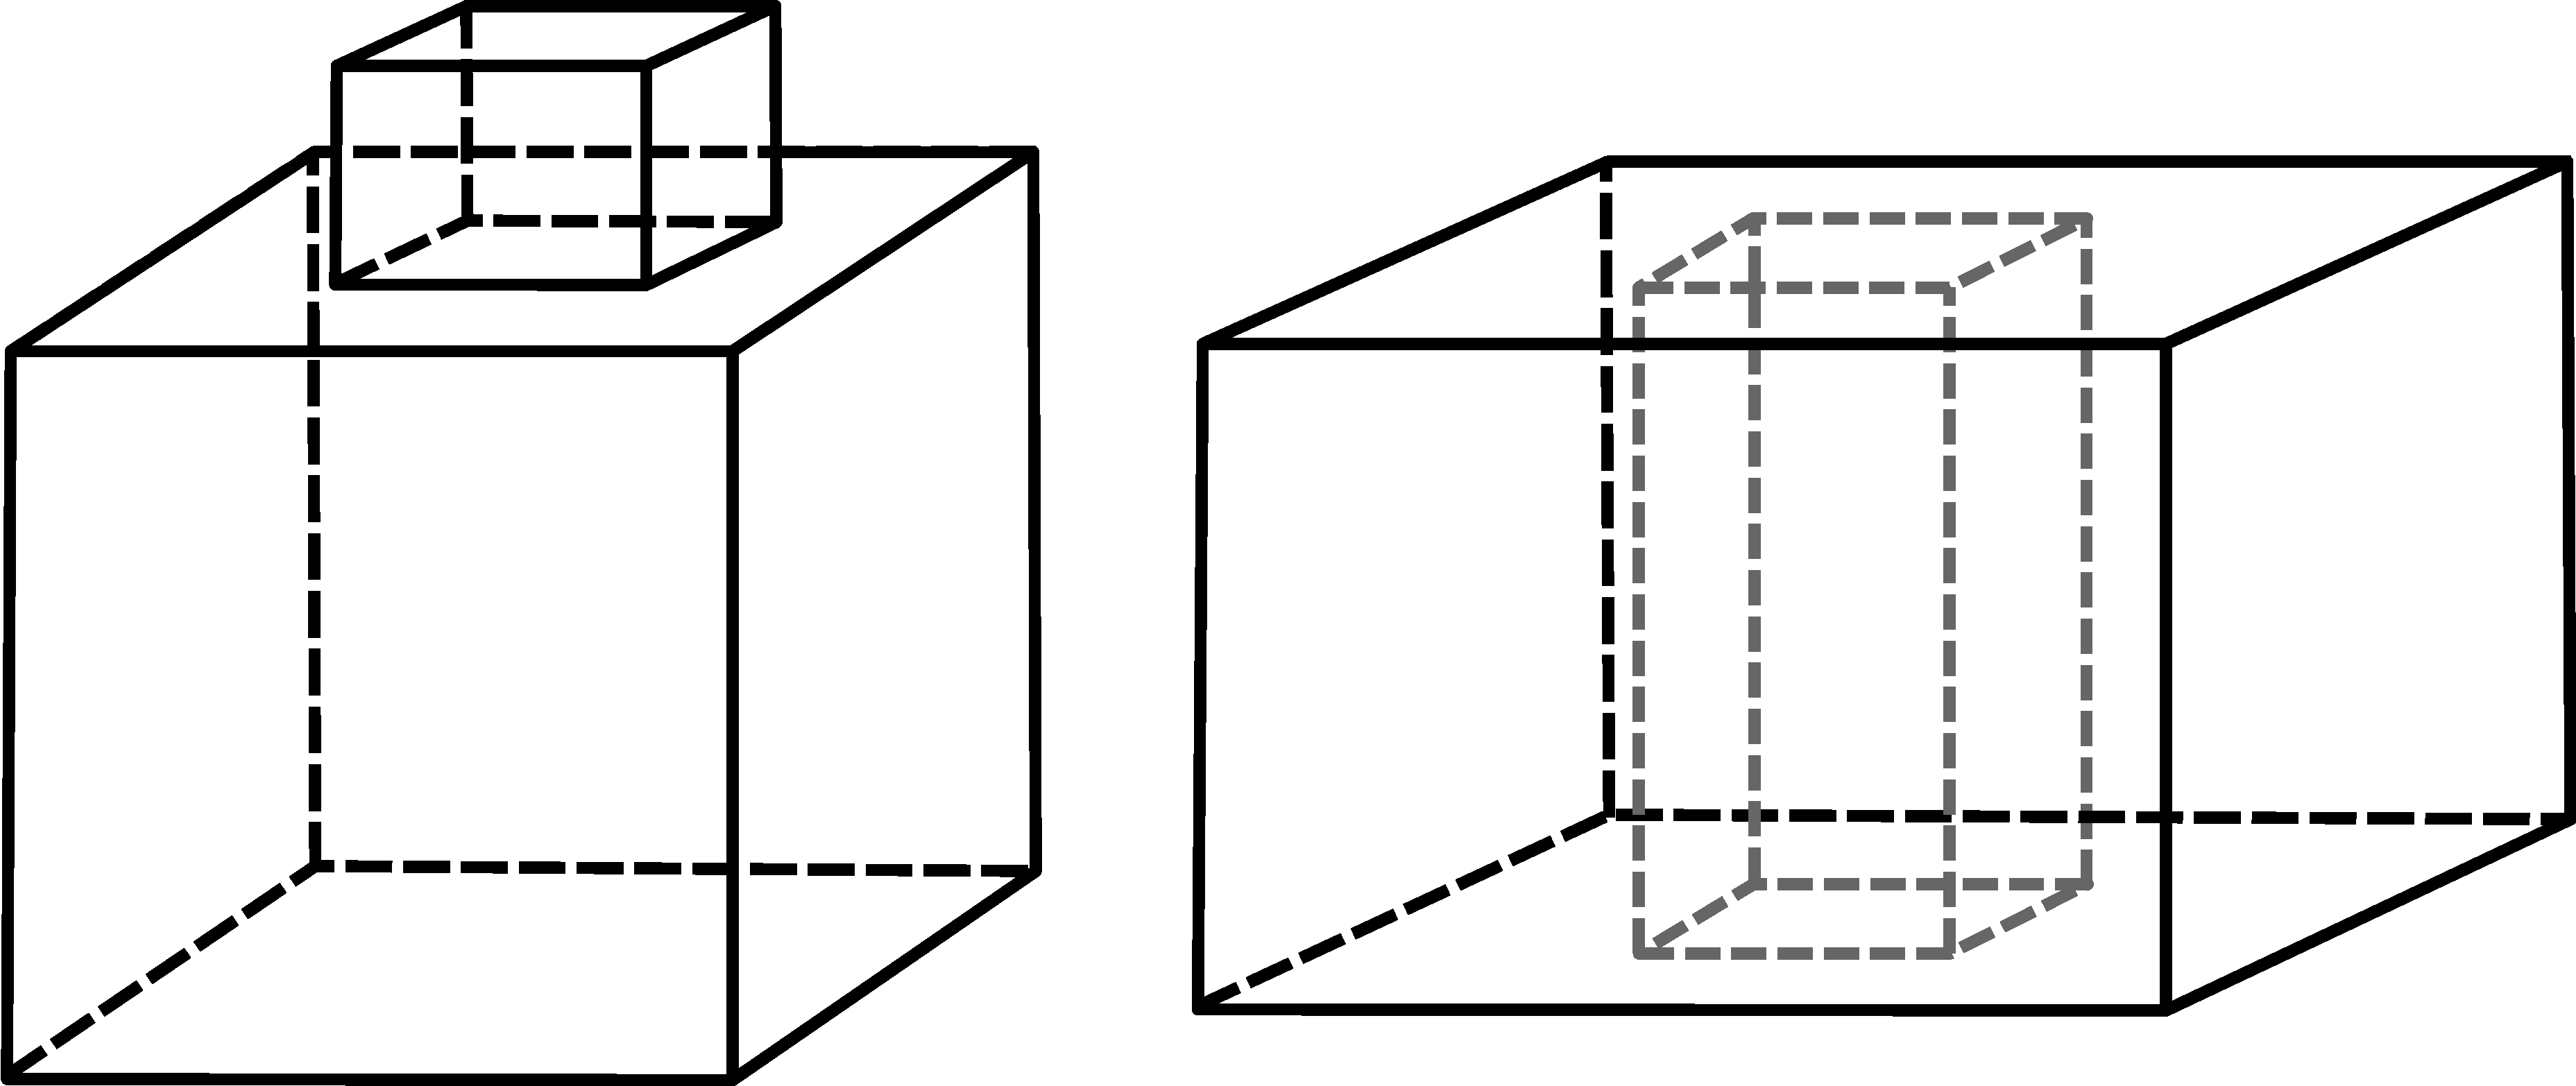
\includegraphics[width=0.6\linewidth]{grafiken/einfache_polyeder_vergleich.pdf}
    \caption{Links ein einfaches und rechts ein nicht-einfaches Polyeder.}
\end{figure}
\begin{defi}[Konvexes Polyeder]
	Ein Polyeder heißt konvex, wenn zu je zwei Punkten aus dem Inneren des Polyeders auch deren Verbindungsstrecke ganz im Polyeder liegt. \citep[51]{Mueller2012}
\end{defi}
\begin{defi}[Reguläres Polyeder]
	Ein konvexes Polyeder heißt regulär, wenn alle Flächen zueinander kongruente regelmäßige Vielecke sind und in jeder Ecke gleich viele Vielecke zusammenstoßen. \citep[51]{Mueller2012}
\end{defi}
Diese Definitionen werden uns erneut im Beweis des Eulerschen Polyedersatzes begegnen. Es gibt genau fünf reguläre Polyeder.\\
\begin{figure}[H]
    \centering
    
\includegraphics[width=0.9\linewidth]{grafiken/platonische_koerper.pdf}
    \caption{Die fünf regulären Polyeder - Tetraeder, Hexaeder, Oktaeder, Dodekaeder und Ikosaeder.}
    \label{fig:grafiken/Platonische_koerper}
\end{figure}
Für diesen Sachverhalt wurden verschiedene Beweise formuliert, von denen wir zwei nachvollziehen bzw. gegenüberstellen wollen. \\
Wir werfen nun zunächst einen Blick zurück in die Geschichte und befassen uns mit der Entdeckung der fünf regulären Polyeder und ihrer Bedeutung im Laufe der Jahrhunderte.\footcite[Die Informationen zur Geschichte stammen von][]{Endl1993} \\
Bereits im antiken Griechenland wurde erkannt und bewiesen, dass nur fünf Platonische Körper existieren: Tetraeder, Hexaeder (Würfel), Oktaeder, Ikosaeder und Dodekaeder. Ihr Namensgeber Platon beschrieb die regulären Polyeder etwa 350 v. Chr. im Kontext des naturphilosophischen, kosmologischen Werks \enquote{Timaios}. Platon war nicht nur von der Vollkommenheit und Symmetrie beeindruckt, sondern insbesondere davon überzeugt, dass vier der Platonischen Körper die Strukturen der Elemente Feuer, Wasser, Erde und Luft beschreiben, aus denen der Kosmos besteht. Der Dodekaeder repräsentierte hingegen die göttlich gegebene Konstellation der Himmelskörper.\\
Die erste Niederschrift der Konstruktion mit Lineal und Zirkel findet sich in Euklids mehrbändigen Werk \textit{Elemente} (Buch XII), das um 300 v.Chr. entstand. Von ihm stammt auch die folgende Begründung, weshalb es nicht mehr als die bekannten fünf Platonischen Körper geben kann:
\begin{proof}
a) Zunächst wollen wir überlegen, warum ein regulärer Polyeder nur aus gleichseitigen Dreiecken, Quadraten oder regelmäßigen Pentagonen bestehen kann. Um überhaupt eine Polyederecke herausbilden zu können, werden mindestens drei Polygone benötigt. \\
Weiter können wir festhalten, dass die Winkelsumme der Kanten, die in der Polyederecke aufeinander treffen, kleiner als der Vollwinkel sein muss, um eine konvexe Ecke zu formen. Anderenfalls, würde die Winkelsumme genau $360^\circ$ betragen, würden die Flächen eine Parkettierung der Ebene bilden. Auch bei mehr als $360^\circ$ wäre hingegen keine Ecke möglich.\\
Die Winkelsumme in regulären n-Ecken kann durch die Formel $(n-2)\cdot 180^\circ$ beschrieben werden (Begründung: Durch das Einzeichnen eines Punktes innerhalb des Polygons kann dieses in Dreiecke unterteilt werden. Die Hinzunahme einer weiteren Ecke erlaubt es uns, genau ein weiteres Dreieck einzuzeichnen. So kann die Zunahme der Winkelsumme um $180^\circ$ mit jeder zusätzlichen Ecke erklärt werden.). Wir erhalten für Dreiecke, Quadrate und regelmäßige Pentagone eine Innenwinkelsumme von $180^\circ, 360^\circ$ bzw. $540^\circ$. Die Winkel in den Ecken sind dementsprechend beim Dreieck $60^\circ$, beim Quadrat $90^\circ$ und im regelmäßigen Fünfeck $108^\circ$ groß. \\
Das regelmäßige Hexagon hat eine Innenwinkelsumme von $720^\circ$, die Winkel in den Ecken messen dementsprechend je $120^\circ$. Drei Hexagone bilden also wegen $3\cdot 120^\circ=360^\circ$ keine konvexe Ecke mehr, natürlich bilden auch vier, fünf, etc. Hexagone keine konvexe Ecke. Auf gleiche Weise sehen wir, dass auch das Aneinanderlegen von drei oder mehr Polygonen mit mehr als sechs Ecken keine konvexe Ecke ergibt.\\
Wir halten fest, dass die Flächen der Platonischen Körper nur regelmäßige Polygone mit drei, vier oder fünf Ecken sein können.\\

b) Jetzt wollen wir überlegen wie viele Dreiecke, Quadrate oder Pentagone an jeweils einer Ecke des Polyeders zusammentreffen können. Wir orientieren uns dabei an obiger Argumentation.\\
Gleichseitige Dreieck besitzen Innenwinkel von $60^\circ$. Wir können bis zu fünf dieser Dreiecke an ihren Ecke zu einer konvexen Polyederecke zusammenfügen. Die auf diese Weise entstehenden Körperecken die durch das Aufeinandertreffen von drei, vier oder fünf Dreiecken entstehen sind  $180^\circ, 240^\circ$ bzw. $300^\circ$ groß.\\
Quadrate besitzen Innenwinkel von $90^\circ$. Um den Vollwinkel nicht zu überschreiten bzw. zu erreichen, können wir nur die Mindestanzahl von drei Flächen aneinanderlegen $(3\cdot90^\circ=270^\circ)$.\\
Gleiches gilt, wenn wir regelmäßige Pentagone als Seitenflächen wählen: Nur drei Fünfecke bilden eine konvexe Ecke, die einen Winkel von $324^\circ$ einschließt.\\
Insgesamt erhalten wir drei Polyeder mit dreieckigen Seitenflächen und jeweils einen mit vier- bzw. fünfeckigen Seitenflächen. Genau genommen wissen wir nun erst, dass es nicht mehr als fünf Platonische Körper geben kann. Die Existenz haben wir nicht explizit nachgewiesen, jedoch kennen wir die Platonischen Körper Tetraeder, Oktaeder und  Ikosaeder (dreieckige Flächen), Hexaeder (viereckige Flächen) und Dodekaeder (fünfeckige Flächen) und damit ist ihre Existenz schließlich auch gesichert.
\end{proof}
Einige Jahrhunderte später fanden die Platonische Körper auch in anderen Disziplinen einen Platz:
Der Astronom Johannes Kepler konstruierte Ende des 16. Jahrhunderts (1596 in Mysterium Cosmographicum) ineinander verschachtelte Modelle der Platonische Körper, um die Umlaufbahnen der bis dato sechs bekannten Planeten (noch unbekannt: Uranus und Neptun) um die Sonne zu beschreiben. Kepler nutzte die Eigenschaft, dass jeder reguläre Polyeder eine Inkugel und eine Umkugel hat. Auf der Inkugel liegen die Mittelpunkte der Seitenflächen des Polyeders, während alle konvexen Ecken auf der Umkugel liegen. Auf diesen Kugelschalen beschreiben die Planeten nach Kepler Kreisbahnen. Die Platonischen Körper passte der Astronom so von innen nach außen zwischen den Kugelhüllen ein, dass eine Kugel die Inkugel des Polyeders ist, während die nächste seine Umkugel ist. Dadurch ergab sich folgende Anordnung: Das Oktaeder lag zwischen Merkur und Venus, das Ikosaeder zwischen Venus und Erde, das Dodekaeder zwischen Erde und Mars, das Tetraeder zwischen Mars und Jupiter und das Hexaeder zwischen Jupiter und Saturn.\footnote{\url{http://www.mathe.tu-freiberg.de/~hebisch/cafe/platonische.html} (10.11.2014)}  Wenngleich Keplers Theorie später widerlegt wurde, war er einer der ersten Naturwissenschaftler, der auf geometrische Sachverhalte zur Erklärung astronomischer Phänomene zurückgriff.\\
Leonhard Euler formulierte im 18. Jahrhundert den Eulerschen Polyedersatz, der eine Aussage über das Verhältnis der Anzahlen an Seitenflächen, Kanten und Ecken macht. Wirklich neu ist das Resultat nicht: Vermutlich wussten auch Descartes im 17. Jahrhundert und der Grieche Archimedes bereits von dem Zusammenhang. Insbesondere brauchen wir den \textit{Eulerschen Polyedersatz}, um den angekündigten zweiten Beweis zur Existenz der fünf Platonischen Körper führen zu können.\\
Verschiedene Vorstellungen von der Konstruktion der Polyeder legen andere Beweisideen zum Eulerschen Poyledersatz nahe, argumentiert Berendonk in seinem Buch "'Erkundungen zum Eulerschen Polyedersatz". \citep[vgl.][39]{Berendonk2014} Der hier geführte Beweis nach von Staudt folgt der Vorstellung, dass Polyeder aus Netzen entstehen.\footnote{Die Beweise von Euler selbst und Cauchy, die Berendonk ebenfalls ausführt und erläutert, sind hingegen am plausibelsten, wenn Polyeder als Festkörper bzw. als aus einzelnen Polygonen zusammengesetzt gedacht werden.}\\
Von Staudt greift in seinem Beweis auf grundlegende Begriffe der Graphentheorie zurück, die wir vorab einführen wollen. Die Graphentheorie als Teilgebiet der Topologie befasst sich mit der Art und Weise, wie Figuren verbunden sind. Die von uns betrachteten Polyeder haben die zentrale Eigenschaft, dass ihre Seitenflächen eine einzige, grenzenlose Oberfläche bilden. Die Kanten sind in diesem Sinne Kurven auf dieser Oberfläche, von denen drei oder mehr dort aufeinander treffen, wo sich die Ecken des Polyeders befinden.
\begin{bem}
Die $N_0$ Ecken und $N_1$ Kanten eines $N_2$-flächigen regelmäßigen, konvexen Polyeders ergeben einen speziellen \textit{Graphen}, der eine Menge aus $N_0$ Punkten bzw. \textit{Knoten} und $N_1$ Segmenten bzw. \textit{Zweigen} ist. Damit ein Graph \textit{zusammenhängend} ist, muss die Ungleichung $N_{1} \geq N_{0}-1$ erfüllt sein.
Einen zusammenhängenden Graphen, der außerdem keine \textit{Zykel} (z.B. durch Polygone) aufweist, nennen wir einen \textit{Baum}. Für Bäume gilt sogar die Gleichung $N_{1} = N_{0}-1$.
\end{bem}
Coxeter fasst die Erkenntnisse wie folgt zusammen: mit anderen Worten ist das Polyeder mit $N_0$ Ecken, $N_1$ Kanten und $N_2$ Flächen ein regulärer Graph, d.h. die $N_1$ Kanten und $N_0$ Ecken schaffen eine Partition der unbegrenzten Oberfläche bestehend aus $N_2$ polygonalen Gebieten \citep[6]{Coxeter1973}.\\
Aus einem gegebenen Graphen können wir einen zweiten ableiten, der auf derselben Oberfläche liegt -- den so genannten \textit{dualen Graphen}.
%\begin{defi}
%Der duale Graph zu einem planaren Graph G ist ein Graph, der zu jeder Fläche von G einen Knoten hat. Außerdem gibt es für jede Kante in G eine Kante im dualen Graph, die in zwei benachbarten Flächen reicht.
%\end{defi}
Die $N_2$ Ecken des dualen Graphen liegen im Inneren der $N_2$ Flächen des Ausgangspolyeders. Außerdem weist der duale Graph $N_1$ Kanten auf, von denen jede jeweils eine Kante des gegebenen Graphen kreuzt. Die $N_0$ Flächen umschließen jeweils eine der $N_0$ Ecken des Ausgangspolyeders. Insbesondere ist die Dualität eine symmetrische Relation: ein Graph ist die Dualität seiner Dualität.\\
Wir können nun Eulers Formel beweisen:
\begin{theorem}[Eulerscher Polyedersatz]
"Bei jedem von ebenen Seitenflächen eingeschlossenen Körper überschreitet die Summe der Zahl der Raumwinkel und der Zahl der Seitenflächen die Zahl der Grate (altdt. Kanten [M.B.]) um zwei."
\end{theorem}
Die heute gebräuchliche Darstellung der Eulerschen Formulierung in algebraischer Formelsprache lautet:
$N_0 - N_1 + N_2 =2 $, wobei $N_0$, $N_1$ und $N_2$ für die Anzahl der Ecken, Kanten und Flächen stehen.
\begin{proof}
Wir betrachten den Baum zur planaren Projektion zu einem Platonischen Körper, der $N_0$ Knoten (Ecken), $N_1$ Kanten und $N_2$ Flächen hat. Die $N_0$ Knoten des Baums sind gerade die Ecken des Platonischen Körpers, es gibt $N_0 -1$ Zweige aus der Menge der $N_1$ Kanten des Polyeders. Anstelle die übrigen Kanten zu nehmen, betrachten wir die entsprechenden Kanten des dualen Graphen. Dieser hat $N_2$ Ecken, die jeweils auch die Mittelpunkte der Flächen des betrachteten Polyeders sind. Die Kanten des dualen Graphen sind unabhängig von denen des beschriebenen Baums und schneiden sie nicht. Der duale Graph ist außerdem zusammenhängend, da die Knoten nur dann separiert wären, wenn ein zum Baum gehörender Zykel im Weg wäre, jedoch ist dies per Definition ausgeschlossen. Andrerseits würde ein Kreislauf im Graphen die Oberfläche in zwei separate Teile zerlegen, was jedoch unmöglich ist. Insgesamt ist der duale Graph also ein zweiter Baum, da er zusammenhängend ist und keine Zykel enthält. Daraus folgt, dass der duale Graph $N_2-1$ Kanten aufweist. Jede Kante des Ausgangspolyeders kann jedoch einem Zweig des ersten oder zweiten Baums zugeordnet werden, da sie entweder einer der Zweige des ersten Baums ist oder von einem der Zweige des zweiten Baums geschnitten wird. Daraus folgt: $N_1 = (N_0-1) + (N_2-1)$, also $N_0 - N_1 + N_2 =2 $.
\end{proof}
Die nachstehenden Abbildungen sind Veranschaulichungen der von Staudtschen Beweisidee für den Hexaeder bzw. den Tetraeder.\\
\begin{figure}[H]
\centering
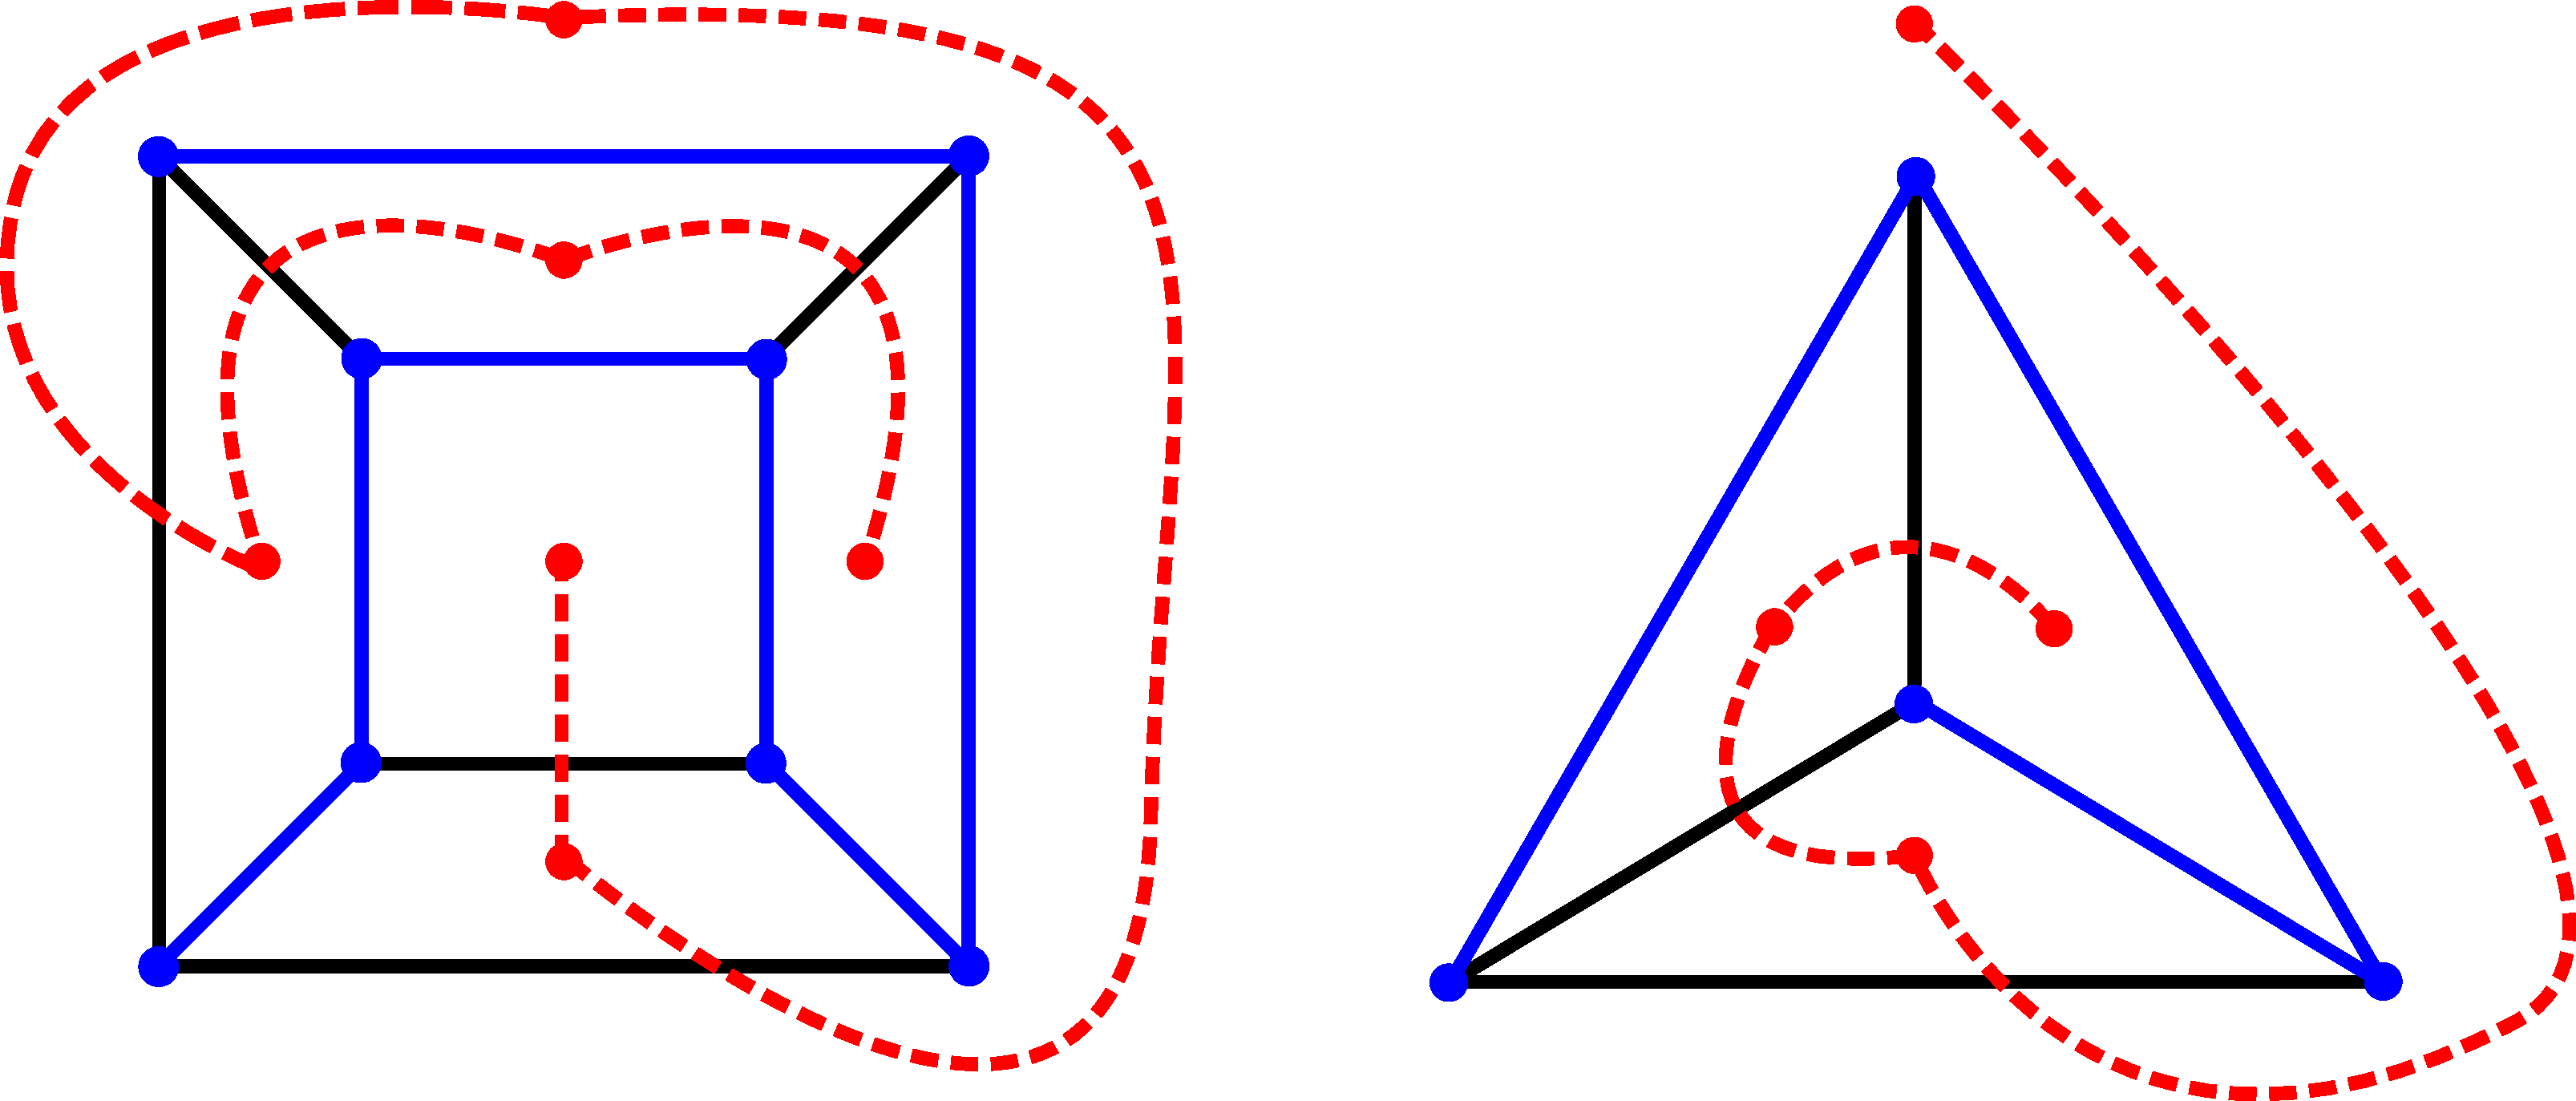
\includegraphics[width=0.7\linewidth]{./grafiken/duale_graphen}
\caption{Veranschaulichung der von Staudtschen Beweisidee}
\label{fig:duale_graphen}
\end{figure}

Der planare Graph des Hexaeders besteht aus einem Quadrat, in das ein kleineres Quadrat symmetrisch einbeschrieben wurde. Die Eckpunkte beider Polygone liegen so auf den eingezeichneten Diagonalen durch den Mittelpunkt.
Die blauen Punkte symbolisieren die acht Ecken des Polyeders bzw. die Knoten des ersten Baums. Die sieben Zweige des Baums sind ebenfalls blau gekennzeichnet. Der duale Graph besteht aus den sechs rot markierten Knoten und den fünf  nicht-durchgezogenen, ebenfalls roten Linien. Der sechste rote Knoten, der anschaulich mit dem Mittelpunkt bzw. einem weiteren roten Knoten zusammenfällt, wurde aus Gründen der Übersichtlichkeit außerhalb des planaren Graphen abgetragen.\\
Der planare Graph zum Tetraeder hat die äußere Form eines gleichseitigen Dreiecks. Die Dreiecksfläche wird punktsymmetrisch vom Mittelpunkt aus mit drei Strecken in drei kongruente Segmente unterteilt. Analog zur Darstellung am Hexaeder sind die Bestandteile des ersten Baums blau hervorgehoben, die des zweiten Graphen rot. Ebenso wurde der vierte Knoten zur Verdeutlichung außerhalb des gleichseitigen Dreiecks abgetragen.
\begin{bem}
Der Eulersche Polyedersatz ist nur für konvexe Polyeder gültig. Man kann sich dessen leicht mit einem Gegenbeispiel für ein nicht-konvexes Polyeder überzeugen.
\end{bem}

Nach dieser Vorbereitung wollen wir nun den zweiten, oben angekündigten Beweis dafür führen, dass es nicht mehr als die fünf uns bekannten regulären Polyeder geben kann:
\begin{proof}
Wir betrachten ein reguläres Polyeder mit $N_2$ Flächen. Jede dieser Flächen ist ein reguläres n-seitiges Polygon.
An jeder der $N_0$ Ecken treffen k Kanten zusammen.
Jede der $N_1$ Kanten gehört zu zwei Flächen. Wenn wir die Kanten nach den Flächen abzählen, ergibt sich:
\begin{align}
\setcounter{equation}{0}
n\cdot N_2= 2\cdot N_1 \label{start1}
\end{align}
Außerdem gehört jede Kante auch zu zwei Ecken. Analog formulieren wir daher:
\begin{align}
k\cdot N_0=2 \cdot N_1 \label{start2}
\end{align}
Der Eulersche Polyedersatz führt beide Gleichungen in einer Formel zusammen:
\begin{align}
\frac{2\cdot N_1}{k} + \frac{2\cdot N_1}{n} - N_1 &= 2 \\
\Leftrightarrow \frac{1}{k} + \frac{1}{n} - \frac{1}{2} &= \frac{1}{N_1}\\
\Leftrightarrow \frac{1}{k} + \frac{1}{n}  &= \frac{1}{N_1} + \frac{1}{2}\label{zusammenfassung}
\end{align}
\end{proof}
Wir wissen einerseits, dass ein Polygon mindestens drei Seiten hat und, dass an jeder Ecke wenigstens drei Flächen zusammentreffen, d.h. es gilt $n\geq 3$ und $k\geq 3$. Andererseits ist die Anzahl Kanten $N_1$ des Polyeders eine natürliche Zahl, sodass die rechte Seite in Gleichung (\ref{zusammenfassung}) größer als $\frac{1}{2}$ ist. Wenn nun auf der linken Seite der Gleichung jedoch $k$ und $n$ größer als 3 wären, könnte die linke Seite insgesamt nicht echt größer als $\frac{1}{2}$  sein. Diese Feststellungen schränken die Zahl der Fälle ein: Wir brauchen nur noch zu untersuchen, welche Werte $k$ bzw. $n$ annimmt, wenn $n=3$ bzw. $k=3$ festgelegt wird.\\
Wir beginnen mit $k=3$.
Gleichung(\ref{zusammenfassung}) kann dann umgeformt werden zu:
\begin{align}
\frac{1}{n}- \frac{1}{6}= \frac{1}{N_1} \label{kfix}
\end{align}
Damit die Differenz echt positiv ist, kann $n$ nur die Werte $3, 4, 5$ annehmen. Dass die Differenz größer 0 sein muss ist klar, da $N_1 \in \mathbb{N}$.
Wenn wir nacheinander $3,4$ und $5$ einsetzen in (\ref{kfix}), erhalten wir für $N_1$ die Werte $6, 12$ und $30$.\\
Fixieren wir $n$ statt $k$, erhalten wir analog diese Gleichung:
\begin{align}
\frac{1}{k}- \frac{1}{6}= \frac{1}{N_1} \label{nfix}
\end{align}
 Dementsprechend kann $k$ ebenfalls nur $3,4$ oder $5$ sein. Die Anzahl der Kanten beträgt wiederum $6, 12$ oder $30$.\\
Im letzten Schritt setzen wir die Werte für $n,k$ und $N_1$ in (\ref{start1}) und (\ref{start2}) bzw. in die Gleichungskette $n\cdot N_2=2\cdot N_1=k\cdot N_0$ ein und erhalten die Werte für $N_0$ und $N_2$. Die Ergebnisse sind in der untenstehenden Tabelle aufgeführt.
\begin{center}
\begin{tabular}{p{4.5cm}|c|c|c}
$n\cdot N_2=2\cdot N_1=k\cdot N_0$ & Anz. Ecken $N_0$& Anz. Flächen $N_2$& Bezeichnung\\ \hline
$3 \cdot N_2=2 \cdot 6=3 \cdot N_0$& 4 & 4 & Tetraeder\\ \hline
$3\cdot N_2=2 \cdot 12=4\cdot N_0$& 8 & 6 & Hexaeder \\ \hline
$3\cdot N_2=2 \cdot 30=5\cdot N_0$& 12 & 20 & Ikosaeder\\ \hline
$4\cdot N_2=2 \cdot 12=3\cdot N_0$& 6 & 8 & Oktaeder \\ \hline
$5\cdot N_2=2 \cdot 30=3\cdot N_0$& 20 & 12 & Dodekaeder

\end{tabular}
\end{center}

\subsection{Klassifikation der endlichen Rotationsgruppen}
Für das folgende Kapitel nehmen wir an, dass $\dim V = 3$ und dass $W$ eine Ebene in $V$ ist. Wenn nun $R$ eine Rotation in $\mathcal{O}(W)$ ist, dann kann $R$ zu einer Rotation in $\mathcal{O}(V)$ erweitert werden, indem wir $Rx=x$ für alle $x \in W^\perp$ setzten und eine Basis ${x_1,x_2,x_3}$ für $V$ wählen mit $x_1 \in W^\perp$, $x_2, x_3 \in W$. Dann wird $R$ durch die Matrix $A$ repräsentiert.
$$A=\begin{pmatrix}
1 & 0 & 0 \\
    0 & \cos{(\theta)} & -\sin{(\theta)} \\
    0 & \sin{(\theta)} & \cos{(\theta)}
\end{pmatrix} $$ 
Zunächst wollen wir uns überlegen, wie wir die zyklische Gruppe und die Diedergruppe ins Dreidimensionale überführen können. Als erstes erweitern wir jede Rotation der zyklischen Gruppe im Zweidimensionalen -- wie oben beschrieben -- in eine Rotation im dreidimensionalen Raum und erhalten so die zyklische Gruppe im dreidimensionalen Raum, die wir mit $\mathcal{C}_3^n$ bezeichnen. 

Um auch die Diedergruppe ins Dreidimensionale zu überführen, müssen wir uns nun damit befassen, wie wir Spiegelungen im zweidimensionalen in den dreidimensionalen Raum überführen können. Wenn eine Spiegelung $S$ aus $\mathcal{O}(W)$ ist, dann erweitern wir sie zu einer Rotation in $\mathcal{O}(V)$ und zwar zu einer Rotation $R$, um den Ursprung mit Winkel $\pi$. Die Spiegelgerade von $S$ wird die Rotationsachse von $R$. Diese Beziehung wollen wir zeigen:
\begin{proof}
    Angenommen, dass $\dim V = 3$ und dass $W$ eine Ebene in $V$ ist. Sei $R \in \mathcal{O}(V)$ eine Rotation um den Winkel $\pi$. Alle Punkte die auf der Rotationsachse liegen, sind Fixpunkte von $R$. Damit die Rotationsachse die ehemalige Spiegelachse der Spiegelung $S$ sein kann, müssen die Fixpunkte der beiden Achsen übereinstimmen. Zunächst bestimmen wir die Fixpunkte von $R$:
	\begin{align*}
        \text{Eig}_R(1) &= \ker{(R-E)} \\
	&= \ker{\begin{pmatrix}
		-2 & 0 & 0 \\
		0 & \cos{\theta} - 1 & \sin{\theta} \\
		0 & \sin{\theta} & -\cos{\theta} -1
		\end{pmatrix}} \\
	&= \ker{\begin{pmatrix}
    1 & 0 & 0 \\
		0 & \sin{\theta}(\cos{\theta} - 1) & \sin^2{\theta} \\
		0 & \sin{\theta}(\cos{\theta} - 1) & (-\cos{\theta} -1)(\cos{\theta} + 1)
		\end{pmatrix}} \\
	&= \ker{\begin{pmatrix}
		1 & 0 & 0 \\
		0 & \sin{\theta}(\cos{\theta} - 1) & \sin^2{\theta} \\
		0 & 0 & -cos^2{\theta}-sin^2{\theta}+1
		\end{pmatrix}} \\
	&= \ker{\begin{pmatrix}
		1 & 0 & 0 \\
		0 & \sin{\theta}(\cos{\theta} - 1) & \sin^2{\theta} \\
		0 & 0 & 0
		\end{pmatrix}} \\
	&= \Span\left\{\begin{pmatrix} 0 \\
	(1 + \cos{\theta}) \\
	\sin{\theta}
	\end{pmatrix}\right\}
	\end{align*}
Jetzt überprüfen wir, ob $S$ in der Ebene dieselben Fixpunkte besitzt, das heißt wir überprüfen, ob $Sx=x$ für alle $x$ aus der Fixpunktmenge von $R$ gilt. Sei $x = r(1+\cos{\theta},\sin{\theta})^T$ mit $r \in \mathbb{R}$.
	\begin{align*}
		Sx &= \begin{pmatrix}
			\cos{\theta} & \sin{\theta} \\
			\sin{\theta} & -\cos{\theta}
		\end{pmatrix}\begin{pmatrix}
		r(1 + \cos{\theta}) \\
		r\sin{\theta}
		\end{pmatrix} \\
		&=	\begin{pmatrix}
		r(1 + \cos{\theta})(\cos{\theta})+r\sin^2{\theta} \\
		r(1 + \cos{\theta})\sin{\theta}+(- \cos{\theta})r\sin{\theta}
		\end{pmatrix} \\
		&=	\begin{pmatrix}
		r(1 + \cos{\theta}) \\
		r\sin{\theta}
		\end{pmatrix}
	\end{align*}
Somit haben wir gezeigt, dass die Fixpunkte der Rotation auch Fixpunkte der Spiegelung sind und damit die Rotationsachse mit der ursprünglichen Spiegelachse übereinstimmt.
\end{proof}
Wenn wir jede Abbildung in einer Diederuntergruppe $\mathcal{H}^n_2$ aus $\mathcal{O}(W)$ zu einer Rotation aus $\mathcal{O}(V)$ erweitern, dann ist die resultierende Menge von Rotationen eine Untergruppe von $\mathcal{O}(V)$, welche isomorph zu $\mathcal{H}^n_2$ ist. Diese Untergruppe nennen wir auch Diedergruppe und bezeichnen sie mit $\mathcal{H}^n_3$.
Nun wollen wir uns mit den Rotationsgruppen der Platonischen Körper beschäftigen. Wenn wir ein reguläres Polyeder um den Ursprung im dreidimensionalen Raum zentrieren, dann bilden die Rotationen aus $\OR{3}$ die das Polyeder wieder in sich überführen eine endliche Untergruppe von $\OR{3}$. Wir können auf die Art und Weise nur drei voneinander unterscheidbare Untergruppen finden, denn die Rotationsgruppen des Würfels und des Oktaeders enthalten die selben Elemente. Genauso verhält es sich mit dem Dodekaeder und dem Ikosaeder. Diesen Zusammenhang können wir uns geometrisch überlegen. Wenn wir die Mittelpunkte benachbarter Seitenflächen des Würfels miteinander verbinden, dann erhalten wir ein in den Würfel einbeschriebenes Oktaeder. Das heißt, dass das Oktaeder unter den Elementen der Rotationsgruppe des Würfels invariant bleibt. Wir hätten auch nach dem selben Prinzip den Würfel in das Oktaeder einbeschreiben können. Bei dem Dodekaeder und dem Ikosaeder können wir ähnlich argumentieren. Schauen wir uns dem Zusammenhang in Abbildung \ref{fig:Dual_Platonische_Koerper} an, wird er noch klarer. 
\begin{figure}[H]
\centering

\includegraphics[width=0.9\linewidth]{grafiken/dual_platonische_koerper.pdf}
\caption{Dualität der Platonischen Körper}
\label{fig:Dual_Platonische_Koerper}
\end{figure}

Jetzt wollen wir uns genauer mit den Rotationsgruppen der Platonischen Körper befassen. Um die folgenden Gedankengänge leichter zu verstehen, kann die Webanwendung \textit{Visualisierung der platonischen Körper}\footnote{\url{http://www-stud.uni-due.de/~simibark/visualisierung-platonische-koerper}} genutzt werden.

Wir nehmen an, dass das Tetraeder am Ursprung ausgerichtet ist, und bezeichnen die Rotationsgruppe, die alle Abbildungen enthält, die das Tetraeder wieder in sich überführen, mit $\mathcal{T}$. Nun müssen wir uns überlegen, welche Rotationen in dieser Untergruppe enthalten sind. Die Tetraedergruppe $\mathcal{T}$ enthält acht Rotationen um die Rotationsachsen zwischen einem Eckpunkt und dem Mittelpunkt der gegenüberliegenden Seite mit Rotationswinkeln $\frac{2}{3}\pi$ und $\frac{4}{3}\pi$, drei Rotationen um die Rotationsachsen zwischen den Mittelpunkten zweier gegenüberliegender Kanten mit Rotationswinkel $\pi$ und die Identität. Es gilt somit $| \mathcal{T} | = 4 \cdot 2 + 3 \cdot 1 + 1 = 12$.

Die Rotationsgruppe des Würfels bezeichnen wir mit $\mathcal{W}$. Die Würfelgruppe $\mathcal{W}$ enthält drei verschiedene Arten von Rotationen und die Identität. Zum einen enthält sie neun Rotationen mit den Winkeln $\frac{1}{2}\pi$ ,$\pi$ und $\frac{3}{2}\pi$ um die Rotationsachsen zwischen den Mittelpunkten zweier gegenüberliegender Seiten, acht Rotationen mit dem Winkeln $\frac{2}{3}\pi$ und $\frac{4}{3}\pi$ um die Rotationsachsen zwischen zwei diagonal gegenüberliegenden Eckpunkten und zuletzt sechs Rotationen mit dem Winkel $\pi$ um die Rotationsachsen zwischen den Mittelpunkten zweier diagonal gegenüberliegender Kanten. Es gilt somit $| \mathcal{W} | = 3 \cdot 3 + 4 \cdot 2 + 6 \cdot 1 + 1 = 24$.

Die Rotationsgruppe $\mathcal{I}$ des Ikosaeders enthält 24 Rotationen um die Rotationsachsen zwischen zwei gegenüberliegenden Eckpunkten mit Rotationswinkel $\frac{2}{5}\pi$, $\frac{4}{5}\pi$, $\frac{6}{5}\pi$, $\frac{8}{5}\pi$, 20 Rotationen um die Rotationsachsen zwischen den Mittelpunkten zweier gegenüberliegender Seiten mit Rotationswinkel $\frac{2}{3}\pi$, $\frac{4}{3}\pi$, 15 Drehungen um die Rotationsachsen zwischen den Mittelpunkten zweier gegenüberliegender Kanten mit Rotationswinkel $\pi$ und der Identität. Es gilt somit $| \mathcal{I} | = 15 \cdot 1 + 10 \cdot 2 + 6 \cdot 4 + 1 = 60$.

Wir haben nun die Rotationsgruppen der zyklischen Gruppe, Diedergruppe und aller regelmäßigen Polyeder bestimmt. Doch bevor wir mit der Klassifizierung der endlichen Rotationsgruppen beginnen können, müssen wir zunächst noch den Begriff des Pols einführen.

\begin{defi}[Pole]
	Wenn $T \in \mathcal{O}(V)$ eine Rotation ausgeschlossen der Identität $E$ ist, dann erhalten wir genau zwei Schnittpunkte der Rotationsachse mit der Einheitskugel um den Ursprung. Diese beiden Punkte nennen wir Pole. Die Menge aller Pole einer Untergruppe $\mathcal{G}$ von $\mathcal{O}(V)$ bezeichnen wir mit $\mathcal{P}$.
\end{defi}

Jetzt können wir die Menge der Pole zu den einzelnen Rotationsgruppen, die wir zuvor diskutiert haben, aufstellen und ihre Mächtigkeit ermitteln. Die zyklische Gruppe $\mathcal{C}^n_3$ enthält $n$ Rotationen, die alle dieselbe Rotationsachse besitzen. Daher besitzt die Polmenge $\mathcal{P}$ zu $\mathcal{C}^n_3$ genau zwei Elemente. Außerdem können wir festhalten, dass kein Pol durch eine Transformation aus $\mathcal{C}^n_3$ auf den anderen überführt wird, daher besitzt $\mathcal{P}$ zwei ein-elementige Bahnen. Wenn wir uns die Bahnformel zur Hilfe nehmen, können wir daraus die Ordnung der Stabilisatoren für die Pole ableiten. Diese kennen wir aus der linearen Algebra und lautet wie folgt:
$$ |G| = |G \circ p| \cdot |G_p| $$
Dabei ist $G \circ p = \{g \circ p | g \in G\}$ die Bahn von $p$ und $G_p = \{g \in G | g \circ p = p \}$ der Stabilisator von $p$.

Wenden wir diese nun auf unser Beispiel an, können wir aus der folgenden Gleichung die Ordnung des Stabilisators ableiten.
\begin{align*}
	 |\mathcal{C}_3^n| &= |\mathcal{C}_3^n \circ p| \cdot |{\mathcal{C}_3^n}_p| \Leftrightarrow\\
	 n &= 1 \cdot |{\mathcal{C}_3^n}_p|
\end{align*}
Jetzt wissen wir, dass die Ordnung des Stabilisators für einen Pol $n$ ist. Als nächstes betrachten wir die Pole der Diedergruppe $\mathcal{H}_3^n$. Diese Gruppe enthält $n$ Rotationen mit verschiedenen Rotationsachsen und eine Rotation, die orthogonal zu den anderen Rotationen steht, demnach enthält die Menge der Pole $\mathcal{P}$ der Gruppe $\mathcal{H}_3^n$ $2n+2$ Pole. Diese Pole kommen auf drei verschiedene Arten zustande. Zum einen erhalten wir Pole von Rotationsachsen die durch die Eckpunkte des Polygons gehen, dann erhalten wir Pole von Rotationsachsen durch die Mittelpunkte der Kanten des Polygons und Pole von der Rotationsachse der Transformationen der zyklischen Gruppe. Zur Veranschaulichung können wir uns die Abbildung angucken.
\begin{figure}[H]
\centering
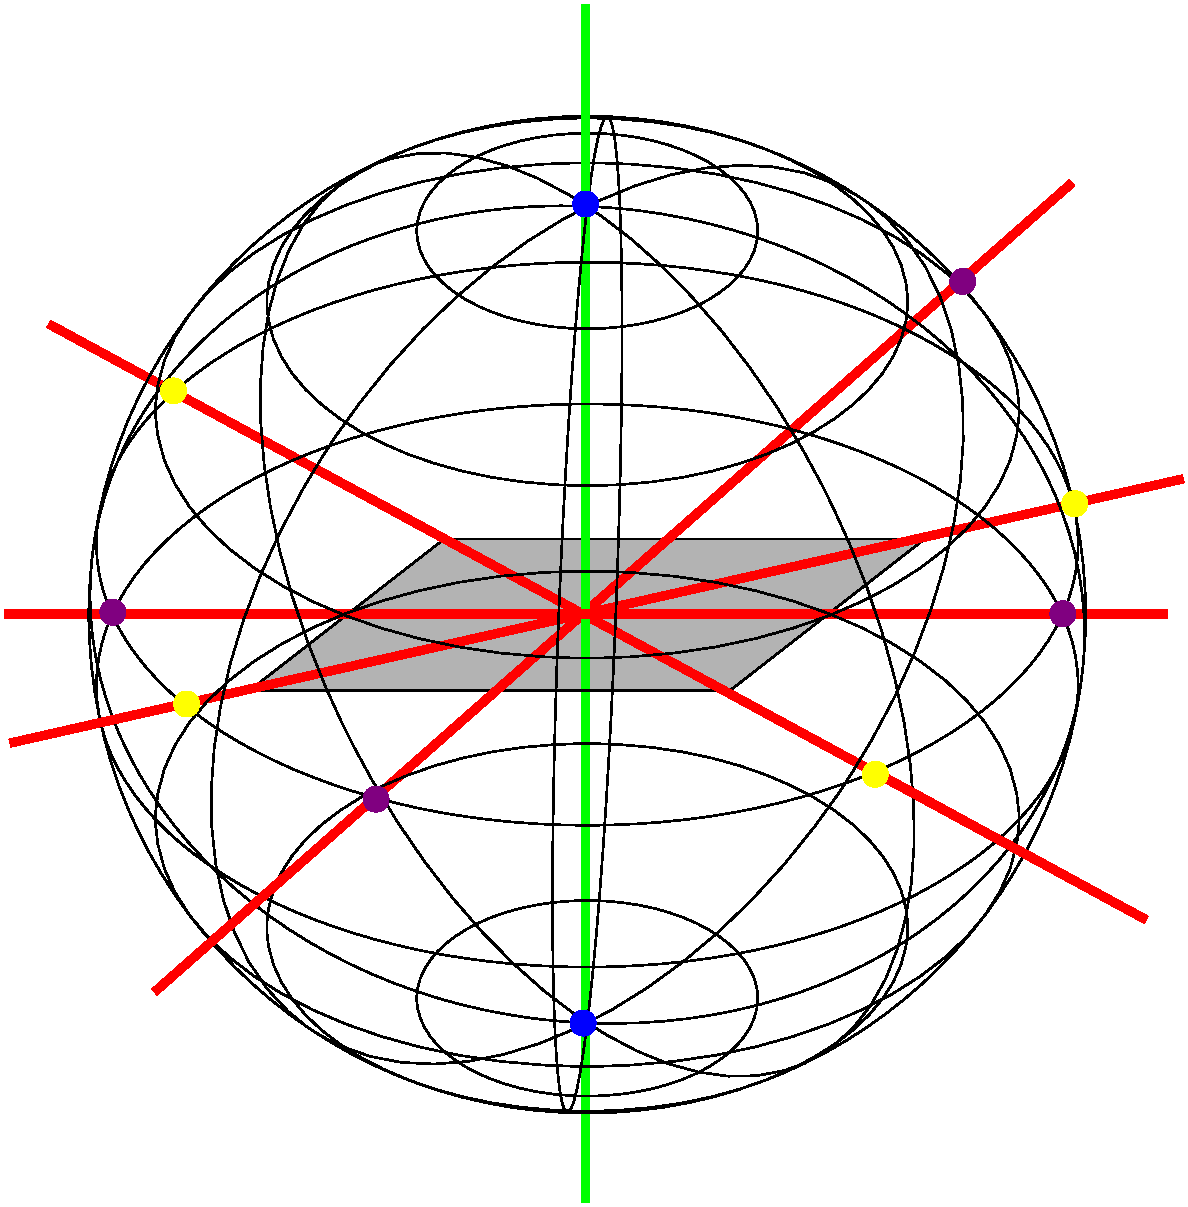
\includegraphics[width=0.5\linewidth]{grafiken/pole_diedergruppe}
\caption{Pole der Diedergruppe $\mathcal{H}_3^4$}
\label{fig:pole_diedergruppe}
\end{figure}
Führen wir dieses Verfahren auch für die platonischen Körper durch, dann erhalten wir folgende Werte:
\begin{center}
	\begin{tabular}{l|cccccc}
		$\mathcal{G}$ & $|\mathcal{G}|$ & $|\mathcal{P}|$ & Anzahl Bahnen & \multicolumn{3}{c}{Ordnung der Stabilisatoren}\\
		\hline
		$\mathcal{C}^n_3$ & $n$ & $2$ & $2$ & \ \ \ \ \ $n$ & \ \ \ \ \ \ $n$ & \\
		$\mathcal{H}^n_3$ & $2n$ & $2n + 2$ & $3$ & \ \ \ \ \ $2$ & \ \ \ \ \ \ $2$ & $n$\\
		$\mathcal{T}$ & $12$ & $14$ & $3$ & \ \ \ \ \ $2$ & \ \ \ \ \ \ $3$ & $3$\\
		$\mathcal{W}$ & $24$ & $26$ & $3$ & \ \ \ \ \  $2$ & \ \ \ \ \ \ $3$ & $4$\\
		$\mathcal{I}$ & $60$ & $62$ & $3$ & \ \ \ \ \ $2$ & \ \ \ \ \ \ $3$ & $5$
	\end{tabular}
\end{center}
Wir behaupten nun, dass wir alle endlichen Rotationsuntergruppen von $\OR{3}$ gefunden haben. Um unsere Behauptung zu festigen, beweisen wir nun den folgenden Satz.
\begin{theorem}
	Haben $\mathcal{C}^n_3,\mathcal{H}^n_3,\mathcal{T},\mathcal{W}$ und $\mathcal{I}$ die gleichen Eigenschaften wie in Bemerkung 5.5, dann ist $\mathcal{C}^n_3,n\geq1;\mathcal{H}^n_3,n\geq2;\mathcal{T};\mathcal{W};\mathcal{I}$ eine komplette Liste aller endlichen Untergruppen von Drehungen aus $\OR{3}$.
\end{theorem}
\begin{proof}
	Sei $\mathcal{G}$ eine endliche Untergruppe bestehend aus Drehungen von $\OR{3}$ und $p \in \mathcal{P}$ ein Pol von $R \in \mathcal{G}$ beliebig, dann sei $Stab(p) := \{R\in \mathcal{G} | R(p)=p\}$ der Stabilisator eines Pols $p$ von $G$ und $R_p := \{R(p) | R \in G \}$ die zugehörige Bahn.

	Zunächst führen wir folgende Bezeichnungen ein
	\begin{center}
		$N:=|\mathcal{G}|$, $n_p:=|\mathcal{G}_p|=$ "`Bahnlänge"', $r_p:=|Stab(p)|$,
	\end{center}
	dann gilt nach der Bahnenformel $N=r_p \cdot n_p$. Nach Definition eines Pols gilt $r_p > 1$, wenn $N > 1$, da die Identität immer in $Stab(p)$ enthalten ist. Außerdem hat $\mathcal{G}$ $r_p - 1$ Elemente mit Pol $p$ nach Definition des Stabilisators. Da jedes $T \in \mathcal{G}\backslash\{E_3\}$ zwei Pole hat, folgt:
	\setcounter{equation}{0}
	\begin{align}
	\sum_{p \in X}(r_p - 1)= 2(N-1)
	\end{align}
	Wenn zwei Pole $p$ und $p^{\#}$ in derselben Bahn liegen, dann folgt $\mathcal{G}_p=\mathcal{G}_{p^{\#}}$ und auch $N=r_p n_p=r_{p^{\#}} n_{p^{\#}}$. Wir können also Summanden von Polen, die in derselben Bahn liegen, zusammenfassen. Wenn gilt $r_i=r_p$, falls $p\in B_i$ die Anzahl der verschiedenen Bahnen $m$ ist, und $n_i:=|B_i|$, dann folgt aus $(1)$
	\begin{align}
	&\sum_{i=1}^m n_i(r_i-1)=2(N-1) \\
	\Leftrightarrow &\underbrace{\sum_{i=1}^m \underbrace{(1-\frac{1}{r_i})}_{\substack{\geq \frac{1}{2}}}}_{\substack{\geq \frac{m}{2}}}=\underbrace{2-\frac{2}{N}}_{\substack{<2}}
	\end{align}
	Aus dieser Gleichung folgt, dass es höchstens 3 Bahnen geben kann, da $m \leq 3$. Wir möchten nun die drei Fälle überprüfen und schauen, welche Drehgruppen wir vorliegen haben.

	\textbf{Fall 1:} Es gilt $m=1$. Also existiert genau eine Bahn und es folgt aus Gleichung (3):
	\begin{align*}
	\underbrace{2-\frac{2}{N}}_{\substack{\geq 1}} = \underbrace{1-\frac{1}{r_1}}_{\substack{<1}}
	\end{align*}
	Dies ist aber ein Widerspruch, sodass es nicht nur eine Bahn geben kann.

	\textbf{Fall 2:} Es gilt $m=2$. Also existieren genau zwei Bahnen und aus (3) folgt:
	\begin{align*}
	2-\frac{2}{N} &= 1-\frac{1}{r_1} + 1-\frac{1}{r_2} \\
	\frac{2}{N} &= \frac{1}{r_1} + \frac{1}{r_2}
	\end{align*}
	Da $N=r_i n_i$ gilt, muss $r_i \leq N$ gelten und somit folgt, dass $r_1 = r_2 = N$ und $n_1 = n_2 = 1$. Beide Bahnen haben die Länge $1$ und daher gibt es nur zwei Pole $p$ und $p^{\#}$. Außerdem liegen sich beide Punkte auf der Einheitskugel gegenüber und sind Fixpunkte von $G$, das heißt die beiden Pole liegen auf einer Gerade durch den Ursprung. Daher kann die Gruppe $G$ nur aus Drehungen um die Drehachse, die von $p$ und $p^{\#}$ gebildet wird, bestehen. Dies ist genau die Eigenschaft der Zyklischen Gruppe, daher gilt $\mathcal{G}=\mathcal{C}_3^n$.
	
	\textbf{Fall 3:} Es gilt $m=3$. Aus (3) folgt dann:
	\begin{align}
	\frac{2}{N} = \frac{1}{r_1} + \frac{1}{r_2} + \frac{1}{r_3} - 1
	\end{align}
	Wir sortieren die Bahnen so, dass $r_1 \leq r_2 \leq r_3$ gilt. Daraus folgt, dass $r_1 = 2$ sein muss, da für $r_i \geq 3$ die rechte Seite sonst kleiner Null wäre und es somit zu einem Widerspruch kommen würde. Mit Hilfe der obigen Gleichung können wir feststellen, dass es nur vier weitere mögliche Kombinationen gibt $\{(2,2,n),(2,3,3),(2,3,4),(2,3,5)\}$.
	
	
	$(2,2,n)$: Aus Gleichung (4) folgt, dass $N = 2n$ und $n_3=2$. Daher besteht die Bahn $B_3$ aus zwei Elementen $p, p^{\#}$. Das heißt, dass jedes Element von $\mathcal{G}$ die Pole $p,p^{\#}$ festhält oder sie vertauscht. Daher müssen sich beide Pole gegenüberliegen und die Elemente aus $\mathcal{G}$ sind entweder Drehungen um die Drehachse $d$ durch die beiden Pole $p,p^{\#}$ oder Drehspiegelungen mit Drehachse $d$ um den Winkel $\pi$ und Spiegelebene $d^{\perp}$. Daher besitzt G genau die Eigenschaften der Diedergruppe und es gilt $\mathcal{G} = \mathcal{H}_3^n$. Die Eckpunkte und die Mittelpunkte der Seiten entsprechen dann den übrigen Polen. 
	
	
	$(2,3,3)$: Aus Gleichung (4) folgt, dass $N = 12$ und $n_1 = 6, n_2 = 4, n_3 = 4$ gilt. Die Pole der Bahn $B_2$ sind die Eckpunkte eines Tetraeders $T$ und $\mathcal{G}$ ist die Drehgruppe $\mathcal{T}$. Außerdem gilt, dass
	\begin{align*}
        n_1 = \# \text{Kanten}(T),n_2 = \# \text{Eckpunkte}(T),n_3 = \# \text{Flächen}(T)
	\end{align*}
	
	
	$(2,3,4)$: Aus Gleichung (4) folgt, dass $N = 24$ und $n_1 = 12, n_2 = 8, n_3 = 6$ gilt. Die Pole der Bahn $B_2$ sind die Eckpunkte eines Würfels $W$ und $\mathcal{G}$ ist die Drehgruppe $\mathcal{W}$. Außerdem gilt, dass
	\begin{align*}
        n_1 = \# \text{Kanten}(W),n_2 = \# \text{Eckpunkte}(W),n_3 = \# \text{Flächen}(W)
	\end{align*}
	
	
	$(2,3,5)$: Aus Gleichung (4) folgt, dass $N = 60$ und $n_1 = 30, n_2 = 20, n_3= 12$ gilt. Die Pole der Bahn $B_3$ sind die Eckpunkte eines Ikosaeders $I$ und $\mathcal{G}$ ist die Drehgruppe $\mathcal{I}$. Außerdem gilt, das
	\begin{align*}
        n_1 = \# \text{Kanten}(I),n_2 = \# \text{Flächen}(I),n_3 = \# \text{Eckpunkte}(T)
	\end{align*}
Somit haben wir alle endlichen Rotationsuntergruppen der orthogonalen Gruppe im dreidimensionalen Raum klassifiziert.
\end{proof}

\subsection{Klassifikation der endlichen orthogonalen Gruppen}
Nachdem wir die endlichen Rotationsgruppen im dreidimensionalen Raum klassifiziert haben, möchten wir nun die endlichen Gruppen klassifizieren. Wir schauen uns zunächst die Gruppe $\mathcal{W}^*$ an. Diese soll alle orthogonalen Abbildungen umfassen, welche den Würfel wieder auf sich selber abbilden. Natürlich ist leicht zu sehen, dass $\mathcal{W}$ kleiner ist als $\mathcal{W}^*$. Aber wir können bemerken, dass für $T \in \mathcal{W}^*\backslash\mathcal{W}$ \ $-T = -1 \cdot T \in \mathcal{W}$ gilt. Daher gilt $\mathcal{W}^*=\mathcal{W}\cup(-1)\mathcal{W}$.
Dieser Eigenschaft lässt sich auf alle Untergruppe von $\mathcal{O}(V)$ generalisieren, egal welche Dimension $V$ besitzt.

\begin{lemma}
    Wenn $\mathcal{G} \leq \mathcal{O}(V)$ und $\mathcal{H}$ Rotationsuntergruppen von $\mathcal{G}$ sind, dann gilt entweder $\mathcal{H}=\mathcal{G}$ oder $[\mathcal{G}:\mathcal{H}] = 2$. Also ist $\mathcal{H}$ ein Normalteiler von $\mathcal{G}$.
\end{lemma}
\begin{proof}
    Sei $T \in \mathcal{G}\backslash\mathcal{H}$. Dann können wir uns ein beliebiges Element $S\in\mathcal{G}\backslash\mathcal{H}$ wählen und es gilt immer $\det(T^{-1}S) = (-1)^2=1$. Daher ist $T^{-1}$ ein Element von $\mathcal{H}$ und es gilt $\mathcal{G} = \mathcal{H} \cup T\mathcal{H}$ und $[\mathcal{G}:\mathcal{H}]=2$.
\end{proof}
Nachdem wir das Lemma bewiesen haben, können wir nun den finalen Satz dieser Ausarbeitung vorbereiten. Wir möchten nun die endlichen Untergruppen der orthogonalen Abbildungen im dreidimensionalen Raum klassifizieren.

Angenommen $\mathcal{H} \leq \mathcal{G}$ sei eine Untergruppe bestehend aus Rotationen von $\mathcal{G}$. Um eine Einteilung zu schaffen, brachten wir drei Fälle.
 
 
 \textbf{Fall 1:} Falls $\mathcal{G} = \mathcal{H}$, dann können wir uns auf die Klassfizierung der endlichen Rotationsgruppen berufen und sind fertig. Wenn dies nicht der Fall ist, dann hat $\mathcal{H}$ den Index $2$ in $\mathcal{G}$.
 
 
 \textbf{Fall 2:} Sei $-E_3 \in \mathcal{G}$, dann gilt $\mathcal{G} = \mathcal{H} \cup - \mathcal{H}$ und $\mathcal{G}$ besteht aus einer Untergruppe die nur aus Rotationen und ihre Negativen besteht.


 \textbf{Fall 3:} Sei $\mathcal{G}\neq \mathcal{H}$, $-E_3 \notin \mathcal{G}$ und $R\mathcal{H}$ ist eine von $\mathcal{H}$ verschiedene Nebenklasse in $\mathcal{G}$. Dann ist $R^2\in\mathcal{H}$, wenn $R^2 \in R \mathcal{H}$ ist und dieses würde bedeuten, dass $R \in \mathcal{H}$. Da $\mathcal{H}$ ein Normalteiler von $\mathcal{G}$ ist folgt, dass $(-R\mathcal{H})(-R\mathcal{H})=R^2\mathcal{H}=\mathcal{H}$. Daher gilt, dass die Menge $\mathcal{K} = \mathcal{H} \cup (-R)\mathcal{H}$ eine Gruppe bestehend aus Rotationen von $\OR{3}$ ist. Dann gilt, dass $\mathcal{G} = \mathcal{H} \cup \{-T:T\in\mathcal{K}\backslash\mathcal{H}\}$ eine Untergruppe von $\OR{3}$ ist, deren Rotationsuntergruppe $\mathcal{H}$ ist. Damit können wir auch die dritte Art von Gruppen klassifizieren, indem wir eine Gruppe der ersten Klasse nehmen, die eine Untergruppe $\mathcal{H}$ von Rotationen mit Index 2 besitzt und dann $\mathcal{G}=\mathcal{H}\cup\{-T:T\in\mathcal{K}\backslash\mathcal{H}\}$ setzen. Die Gruppe bezeichnen wir dann mit $\mathcal{K}]\mathcal{H}$.


\begin{theorem}
 Sei $\mathcal{G}\leq\OR{3}$, dann ist $\mathcal{G}$ isomorph zu einer der folgenden Klassen:
 \begin{itemize}
  \item $\mathcal{C}^n_3,n\geq1;\mathcal{H}^n_3,n\geq2;\mathcal{T};\mathcal{W};\mathcal{I}$
  \item $(\mathcal{C}^n_3)^*,n\geq1;(\mathcal{H}^n_3)^*,n\geq 2;\mathcal{T}^*;\mathcal{W}^*;\mathcal{I}^*$
  \item $\mathcal{C}^{2n}_3]\mathcal{C}^n_3,n\geq1;\mathcal{H}^n_3]\mathcal{C}^n_3,n\geq 2;\mathcal{H}^{2n}_3]\mathcal{H}^n_3,n\geq2;\mathcal{W}]\mathcal{T}$
\end{itemize}
Hinweis: $\mathcal{R}^*:=\mathcal{R}\cup -\mathcal{R}$ und $\mathcal{R}]\mathcal{P}:=\mathcal{P}\cup \{-U|U\in \mathcal{R} \backslash \mathcal{P} \}$
\end{theorem}
Nun haben wir eine komplette Auf"|flistung aller endlichen Untergruppen der orthogonalen Gruppe im dreidimensionalen Raum gefunden. Was wir uns jetzt noch überlegen müssen ist, ob diese Liste keine redundanten Elemente enthält.



\newpage
\nocite{Grove1985}
\printbibliography[title=Literaturverzeichnis]
\newpage
\section*{Eigenständigkeitserklärung}
Hiermit bestätige ich, dass ich die vorliegende Arbeit selbständig verfasst
und keine anderen als die angegebenen Hilfsmittel benutzt habe. Die Stellen
der Arbeit, die dem Wortlaut oder dem Sinn nach anderen Werken (dazu zählen
auch Internetquellen) entnommen sind, wurden unter Angabe der Quelle kenntlich
gemacht.

\vspace{3cm}
\noindent
\underline{\hspace{4cm}}\hfill\underline{\hspace{6.6cm}}\\
Ort~~~~~Datum\hfill Unterschrift\hspace{4cm}

\addcontentsline{toc}{section}{Eigenständigkeitserklärung}
\end{document}
